\newif\iflonger
\longerfalse

\newif\ifolder
\olderfalse


\def\Figurespath{./data/MA}

%In this chapter we consider massive multiple access problem where the access point is only interested in recovering the set of messages. 

%We propose a novel coding scheme for the unsourced multiple access channel model introduced by Polyanskiy~\cite{polyanskiy2017perspective}.
%This new paradigm is composed of four main ingredients: (i) the transmission period is partitioned into sub-blocks, thereby instituting a slotted framework; (ii) The message (data) is split into two parts and one part chooses an interleaver for a low density parity check (LDPC) type code. This part of the message is encoded using spreading sequences or codewords that are designed to be decoded by a compressed sensing type decoder; (iii) The other part of the message is encoded using a low density parity check (LDPC) type code and decoded using a joint message passing decoding algorithm designed for the $T$-user binary input real adder channel;
%(iv) users repeat their codeword in multiple sub-blocks, with the transmission pattern being a deterministic function of message content and independent of the identity of the user. When this coding scheme is combined with successive interference cancellation, the ensuing communication infrastructure can offer significant performance improvements compared to the recently proposed coding scheme in \cite{ordentlich2017low} and results in the best performing coding scheme to date.

%--------------------------------------------------------------------------
%\section{Introduction}
In~\cite{polyanskiy2017perspective}, Polyanskiy introduced an interesting and timely multiple access problem; throughout, we refer to this new formulation as the unsourced multiple access channel model (MAC). In this setting, a very large number, $\Ktot$, of users in a wireless network operate in an uncoordinated fashion. Out of the $\Ktot$ users, a subset of $\Ka$ users are active at any time; and each of them wishes to communicate a $B$-bit message to a central base station. The base station is interested only in recovering the list of messages without regard to the identity of the user who transmitted a particular message. In addition to this, the interest is typically in the case when $B$ is small.

The unsourced, uncoordinated nature of the problem and the small block lengths represent a substantial departure from the traditional multiple access channel and, consequently, has important implications both on the fundamental limits as well as the design of pragmatic low-complexity coding schemes. Due to small block lengths, information rates do not provide reasonable benchmarks and finite block length bounds are more meaningful. In \cite{polyanskiy2017perspective}, Polyanskiy provides bounds on the performance of finite-length codes for this channel model.
%
The design of coding schemes is also very challenging for this setting. Almost all well-known low-complexity coding solutions for the traditional MAC channel such as code-division multiple access, rate-splitting \cite{rimoldi1996rate}, and interleave-division multiple access \cite{ping2006interleave}, implicitly assume some form of coordination between the users and that some parameters of the coding scheme such as the spreading sequence, code rates, time sharing parameters, Tanner graph of the code, etc., are user dependent. When the message length is small, establishing such coordination becomes inefficient; this renders well-known coding solutions tailored to the traditional MAC inadequate for the unsourced MAC. Ordentlich and Polyanskiy describe the first low-complexity coding paradigm for the unsourced MAC~\cite{ordentlich2017low}. In their scheme, a transmission period is partitioned into smaller sub-blocks and users randomly pick one sub-block to transmit in. The encoding structure employed by each user is a concatenated code where the inner code is designed to recover the modulo-$p$ sum of codewords transmitted by users and the outer code is designed to decode multiple users given the modulo-$p$ sum of their codewords. Succinctly, the inner code operates in the spirit of integer-forcing \cite{zhan2014integer}, whereas the outer code is an optimal code for the $T$-user modulo-$p$ multiple access channel~\cite{mathys1990class}.

While Ordentlich and Polyanskiy have contributed an important first step in finding practical schemes for the unsourced MAC, there remains a substantial gap between the performance of their proposed scheme and the capacity limit derived in~\cite{polyanskiy2017perspective}. Indeed, they point to this gap and discuss possibilities for improving its performance. In \cite[Section~III.A]{ordentlich2017low}, they discuss the possibility of improving their scheme by decoding the $T$ messages using the real sum from the channel output instead of first reducing the output of the channel to modulo-$p$ operations. However, in the unsourced MAC, each user is forced to use the same codebook and they remark that ``the task of designing low complexity capacity approaching same-codebook schemes for the real binary adder seems quite challenging.'' Another important limitation that is not discussed in \cite{ordentlich2017low} is that their scheme does not admit iterative cancellation and, hence, successive interference cancellation is not considered.
Therefore, when more than $T$-users transmit in a slot, this slot is not utilized in the decoding process. As a result, their scheme uses a large number of slots in order to ensure that every user is received in a time slot that contains at most $T$-users, resulting in poor spectral efficiency.

The main contribution of this chapter is to propose, analyze and optimize a new coding architecture that overcomes these drawbacks and substantially improves performance when compared to the state-of-the-art.
Key features of our scheme are summarized as follows.
\begin{itemize}
\item \textbf{User Symmetry:} Active users employ the same coding scheme, with transmitted signals determined solely by the message to be transmitted and is independent of the identity of the user. To be precise, no parameter of the encoding scheme such as the interleaver and spreading sequence are unique to a transmitter.
\item \textbf{Binary-input, real-adder channel:}
The proposed coding scheme is tailored to the binary-input real-adder channel.
The information message is split into two parts.
The first portion picks an interleaver for an LDPC code, and the second part is encoded using this LDPC code.
Bits associated with the first portion are communicated using a compressed sensing scheme.
The second part is decoded using a message passing decoder that jointly recovers up to $T$ messages within a slot.
\item \textbf{Successive interference cancellation:} Active users repeat their codewords in several slots. The repetition patterns are selected based on message bits. This scheme facilitates interference cancellation within the slotted structure, and therefore renders obsolete the over-provisioning of slots to avoid undue collisions with more than $T$ users.
\end{itemize}
While \cite{ordentlich2017low} also incorporates the user symmetry aspect described above, our scheme differs from theirs in the other features highlighted above.


\begin{table}[!ht]
\centering
\begin{tabular}{|c|l|}
\hline
Notation & Parameter represented\\
\hline
$\Ktot$ & Total number of users in the system\\
$\Ka$ & Number of active users\\
$\tilde{N}$ &  Number of channel uses per frame\\
$\epsilon$ & Maximum decoding probability of error, per active user\\
$V$ & Number of slots each frame is divided into\\
$N$ & Number of channel uses per slot i.e. $N=\tilde{N}/V$\\
$B$ & Number of message bits each active user wants to transmit\\
$\Np,\Nc$ & Channel uses allocated for preamble and channel coding respectively.\\
		& Note that  $\Np+\Nc=N$ \\
$\Bp,\Bc$ & Message bits transmitted by the preamble and channel coding \\
       & components respectively. Note that $\Bp+\Bc=B$\\
\hline
\end{tabular}
\caption{Important parameters encountered in this chapter along with the notation used are listed above.}
\label{table:notaiton}
\end{table}

\section{System model}
The observed signal vector at the receiver corresponding to the $\tilde{N}$ channel uses can be written as
\begin{equation}
\yv = \sum_{i=1}^{\Ktot} s_i \xv_{i} + \zv,
\end{equation}
where $\xv_i$ is a signal of dimension $\tilde{N}$ transmitted by the user~$i$, and the additive noise is characterized by $\zv \sim \mc{N}(0,\mathbf{I}_{\tilde{N}})$. For convenience, we use boolean indicators indexed by $i$, where $s_i =1$ if user~$i$ is active and $s_i = 0$ otherwise. We impose an average power constraint on the transmitted vectors when averaged over all possible message indices, i.e., $\frac{1}{M}\sum_{w} ||\xv(w)||^2\leq \tilde{N}P$.  The receiver produces a list of messages $\mc{L}(\yv) = \{\hat{w}_1,\hat{w}_2,\ldots,\hat{w}_{\Ka} \}$. As in \cite{ordentlich2017low}, the probability of decoding error, per active user, is defined as
\begin{equation}\label{eqn:proboferrordefinition}
  P_e = \max_{|(s_1,\ldots,s_{\Ktot})| = \Ka} \frac{1}{\Ka} \sum_{i=1}^{\Ktot} s_i \Pr\left( w_i \notin \mc{L}(\yv) \right)
\end{equation}
where $|\cdot|$ denotes the Hamming weight. The objective of the problem is to design a coding scheme with polynomial encoding and decoding complexities such that $P_e \leq \epsilon$ for a given per user target error rate $\epsilon$.

\section{Description of the proposed scheme}
The overall schematic of the proposed scheme is shown in Fig.~\ref{fig:overallscheme}. In our proposed scheme, the $\tilde{N}$ channel uses which are available for communication are split into $V$ sub-blocks (also referred to as slots throughout the chapter), each of length $N=\tilde{N}/V$ channel uses. The encoding operation at the $i$-th user takes place in two steps.

\begin{figure}[h]
  \centering
  \resizebox{0.9\textwidth}{!}{\begin{tikzpicture}

\def\nodewidth{0.5in}
\def\fsize{\Large}
\def\sfsize{\normalsize}
\def\xoffs{0.5in}
\def\ya{3.5}
\def\xr{4}
\def\xslots{11}
\def\xdec{18}
\tikzstyle{block} = [rectangle, draw, thick, opacity=0.7,line width =2, minimum size=\nodewidth]
\tikzstyle{vertRectangle} = [rectangle, draw, opacity=0.7,line width =2, minimum width=\nodewidth, minimum height=12*\nodewidth]
\tikzstyle{opnode} = [rectangle, draw, thick,opacity=0.7,line width=1, minimum size=0.2in]

\node[block] (r11) at (-0.5,0){\fsize \textbf{Encoder} $\mc{C}$};
\node[block] (r21) at (\xr,0) {\fsize \begin{tabular}{c}
Repeat \\
$\ell_{w_1}$ times
\end{tabular}};

\node[block] (r12) at (-0.5,-\ya){\fsize \textbf{Encoder} $\mc{C}$};
\node[block] (r22) at (\xr,-\ya) {\fsize \begin{tabular}{c}
Repeat \\
$\ell_{w_i}$ times
\end{tabular}};

\node[block] (r13) at (-0.5,-3*\ya){\fsize \textbf{Encoder} $\mc{C}$};
\node[block] (r23) at (\xr,-3*\ya) {\fsize 
\begin{tabular}{c}
Repeat \\
$\ell_{w_{K_a}}$ times
\end{tabular}};

\node[vertRectangle] (r3) at (\xslots,-1.5*\ya){\fsize \bf Slots};
\node[vertRectangle,align=center] (r4) at (\xdec,-1.5*\ya){\fsize \bf \begin{tabular}{c}
Up to T-users\\
jointly decoded \\ 
 in each slot\\
+ \\ 
Successive Interference \\
Cancellation (SIC) \\
across slots.
\end{tabular}
};

\draw[<-, thick, line width=2] (r11.west)--node[midway, above]{\fsize $w_1$}+(-\xoffs,0);
\draw[->, thick, line width=2] (r11.east)--node[midway, above]{\fsize $\xv_{w_1}$}(r21.west);

\draw[<-, thick, line width=2] (r12.west)--node[midway, above]{\fsize $w_i$}+(-\xoffs,0);
\draw[->, thick, line width=2] (r12.east)--node[midway, above]{\fsize $\xv_{w_i}$}(r22.west);

\draw[<-, thick, line width=2] (r13.west)--node[midway, above]{\fsize $w_{K_a}$}+(-\xoffs,0);
\draw[->, thick, line width=2] (r13.east)--node[midway, above]{\fsize $\xv_{w_{K_a}}$}(r23.west);

\draw[transform canvas={yshift=-\nodewidth},thick] (r3.north west) -- (r3.north east);
\draw[transform canvas={yshift=-2*\nodewidth},thick] (r3.north west) -- (r3.north east);
\draw[transform canvas={yshift=-3*\nodewidth},thick] (r3.north west) -- (r3.north east);
\draw[transform canvas={yshift=\nodewidth}] (r3.south west) -- (r3.south east);
\node [below=0.3*\nodewidth of r3.north](s1) {\fsize Slot 1};
\node [below=1.3*\nodewidth of r3.north](s2) {\fsize Slot 2};
\node [below=2.3*\nodewidth of r3.north](s3) {\fsize Slot 3};
\node [above=0.3*\nodewidth of r3.south](s4) {\fsize Slot V};
\node [below=3.5*\nodewidth of r3.north]() {\Huge $\vdots$};
\node [above=3.5*\nodewidth of r3.south]() {\Huge $\vdots$};


\begin{scope}[very thick,decoration={
    markings,
    mark=at position 0.5 with {\arrow{>}}}
    ] 
\draw[transform canvas={yshift=-0.5*\nodewidth},postaction={decorate}] (r3.north east) -- (r4.north west);
\draw[transform canvas={yshift=-1.5*\nodewidth},postaction={decorate}] (r3.north east) -- (r4.north west);
\draw[transform canvas={yshift=-2.5*\nodewidth},postaction={decorate}] (r3.north east) -- (r4.north west);
\draw[transform canvas={yshift=0.5*\nodewidth},postaction={decorate}] (r3.south east) -- (r4.south west);
\end{scope}

\draw[<-, thick] (r3.north west)++(0,-2.5*\nodewidth)--(r21.east);
\draw[<-, thick] (r3.north west)++(0,-9.5*\nodewidth)--(r21.east);
\path (r21.east) -- ++(5:0.5cm) coordinate(r21a) 
		  (r21.east) -- ++(320:0.5cm) coordinate(r21b) ;
%\draw[<->,thick] (r21a) to [bend left=30] (r21b) node [right] {\fsize $L_{w_1}$};

\draw[<-, thick] (r3.north west)++(0,-2.5*\nodewidth)--(r22.east);
\draw[<-, thick] (r3.north west)++(0,-1.5*\nodewidth)--(r22.east);
\draw[<-, thick] (r3.north west)++(0,-8.5*\nodewidth)--(r22.east);
\path (r22.east) -- ++(25:0.5cm) coordinate(r22a) 
		  (r22.east) -- ++(335:0.5cm) coordinate(r22b) ;
%\draw[<->,thick] (r22a) to [bend left=30] (r22b) node [right] {\fsize $L_{w_i}$};


\draw[<-, thick] (r3.north west)++(0,-0.5*\nodewidth)--(r23.east);
\draw[<-, thick] (r3.north west)++(0,-6.5*\nodewidth)--(r23.east);
\path (r23.east) -- ++(22:0.5cm) coordinate(r23a) 
		  (r23.east) -- ++(55:0.5cm) coordinate(r23b) ;
%\draw[<->] (r23a) to [bend right=30] (r23b) node [right] {\fsize $L_{w_{K_a}}$};


\draw[->, thick, line width=2] (r4.east)--node[midway, above]{\fsize $\widehat{w}_1,\ldots, \widehat{w}_{K_a}$}+(2.5*\xoffs,0);
\end{tikzpicture}}
  \caption{Schematic of the proposed scheme}
  \label{fig:overallscheme}
\end{figure}

\subsection{Transmission policy across sub-blocks - message based repetition}
\label{sec:Txpolicy_TannerGraph}
For the code word to be transmitted in a sub-block each user uses an identical code book (not-necessarily linear) $\mc{C}$ of rate $\frac{B}{N}$ and length $N$. Given the message index to be transmitted is $w_i$ the user encodes it into a codeword $\cv_{w_i} \in \mc{C}$ and modulates $\cv_{w_i}$ into $\vec{x}_{w_i}$. In the following discussion, we will refer to $\cv_{w_i}$ as the transmitted codeword and the reader should assume that the codeword is modulated appropriately and transmitted. Each user also chooses a repetition parameter $\ell_{w_i}=g(w_i)$ using a function $g:[1:M] \rightarrow [1:V]$ and repeats their codeword $\cv_{w_i}$, $\ell_{w_i}$ times by choosing $\ell_{w_i}$ sub blocks from $[1:V]$ based on the message $w_i$ and transmits during these sub blocks. It is important to note that $\ell_{w_i}$ as well as the slots where the codeword is repeated are deterministic functions of the message index and do not depend on the identity of the user. As shown in Fig.~\ref{fig:overallscheme}, a Tanner graph $G$ can be used to visualize the repetition of the codewords where the left nodes correspond to users and the right nodes corresponds to sub-blocks. The degree of the left nodes is determined by $\ell_{w_i}$ and choosing $w_i$ uniformly at random induces a distribution on $\ell_{w_i}$ through the function $g$.  Let the left degree distribution (d.d) from node perspective be $L(x) = \sum_{{i=1}}^{{l_{\max}}} L_i x^i$, where $L_i$ denotes the fraction of user (left) nodes that are connected to $i$ slot(right) nodes. Similarly let the left d.d from edge perspective be denoted by $\lambda(x) = \sum_{{i=1}}^{{l_{\max}}} \lambda_i x^{i-1}$, where $\lambda_i$ denotes the fraction of edges in $G$ that are connected to left nodes connected to $i-1$ other edges. The two distributions $L(x)$ and $\lambda(x)$ are related as $L(x)=\frac{L'(x)}{L'(1)}$. We choose the mapping $g$ such that a desired left d.d. $L(x)$ (or equivalently $\lambda(x)$) is obtained.

During the $j$-th sub-block, let $\mc{N}_j$ denote the set of users who transmit. During the $j$-th sub-block, the $i$-th user transmits symbols of positive power if $i \in \mc{N}_j$. Otherwise, the $i$-th user remains silent. The received signal during the $j$-th sub-block is given by
\begin{equation}
\yv_j = \sum_{i\in \mc{N}_j} \xv_{w_i} + \zv_j.
\end{equation}

\subsection{Transmission policy within a sub-block - same code book scheme for the $T$-user multiple access}
There are two components to the code $\mc{C}$ used in the proposed transmission scheme within each sub-block: a good sensing matrix for a $T$-sparse robust compressed sensing (CS) problem and a good channel code for the $T$-user binary-input real-adder channel that is decodable with low computational complexity. The $B$ bits to be transmitted are split into two groups of size $B_{\mathrm{p}}$ and $B_{\mathrm{c}} = B-B_{\mathrm{p}}$ bits, respectively. For convenience, we define $M_{\mathrm{p}} \coleq 2^{B_{\mathrm{p}}}$ and $M_{\mathrm{c}} \coleq 2^{B_{\mathrm{c}}}$. The main idea is to use a linear code $\mc{C}_{\textrm{c}}$ good for multiple access channel coding to encode $B_{\mathrm{c}}$ message bits which we refer to as channel coding message bits. The remaining $B_{\mathrm{p}}$ bits, which we refer to as preamble message bits, are used to pick a permutation of the codeword belonging to the channel code $\mc{C}_{\textrm{c}}$ encoded using the $\Bc$ channel coding message bits. Typically, we want $B_{\mathrm{p}} \ll B_{\mathrm{c}}$.

For the channel coding part of the code book $\mc{C}$ we begin with a good linear block code such as a low density parity check (LDPC) code or a spatially-coupled low density parity check (SCLDPC) code $\mc{C}_\text{c}$ of rate $\frac{B_\mathrm{c}}{\Nc}$ and length $\Nc$. As an example, we will consider the case when $\mc{C}_{\text{c}}$ is chosen uniformly at random from the $(\sf{l,r,w},\Nc)$ SCLDPC ensemble \cite{kudekar2011threshold}. Let the modulated codewords of $\mc{C}_{\text{c}}$ be denoted by $\{\cv_1,\cv_2,\ldots,\cv_{M_\mathrm{c}} \}$, where $\cv_{w} = [c_{w}(1),c_{w}(2),\ldots,c_{w}(\Nc)]$,  $c_{w}(i)\in\{\pm\sqrt{\Pc}\}~\forall i$ satisfying the power constraint
\begin{align}
||\cv_w||_2^2= \Nc \Pc
\label{eqn:mac_powerconstraint}
\end{align}
denotes the modulated SCLDPC codeword corresponding to message index $w$. 

For the second part of the encoder let $\mathbf{A}\in\{-\sqrt{\Pp},+\sqrt{\Pp}\}^{\Np\times M_\mathrm{p}}$ denote a sensing matrix that can recover the sum of any $T$ columns of $\mathbf{A}$ with low error probability. Let $f:[1:M_\mathrm{p}] \rightarrow [1:\Nc!]$ denote a hash function which maps $B_\mathrm{p}$  preamble message bits into an integer $\tau_w = f(w)$ such that $\tau_w$ is uniformly distributed over $[1:\Nc!]$ denoting all possible permutations of length $\Nc$. Note that here the integer $\tau_w$ chooses the permutation $\pi_{\tau_w}\in S_{\Nc}$ of the encoded codeword from $\mc{C}_{\text{c}}$ before transmission where $S_{\Nc}$ is the symmetric group.

The description of the overall encoder for code book $\mc{C}$ combining the above two components can be described as following. Let $w= (\wpdash,\wc)$ be the message index to be encoded, where the indices $\wpdash$ and $\wc$ correspond to the preamble and coding message indices respectively. We first encode the message index $\wc$ to the codeword $\cv_{\wc}\in\mc{C}_{c}$ followed by permuting it according to permutation $\pi_{\tau_{\wpdash}}=[\pi_{\tau_{\wpdash}}^1,\pi_{\tau_{\wpdash}}^2,\ldots, \pi_{\tau_{\wpdash}}^{\Nc}]$. The final code word $\cv_{w}$ is then obtained by inserting the $\wpdash$th column from the compressed sensing matrix $\mathbf{A}$ at the beginning of the permuted codeword i.e.,
\begin{align}
  \cv_w &= [\av_{\wpdash},\pi_{\tau_{\wpdash}}(\cv_{\wc})]  \qquad \qquad \text{ where }  \av_{\wpdash} \in \mathbf{A}, \cv_{\wc}\in\mathcal{C}_{\text{c}} \notag \\
&= [\av_{\wpdash},c_{\wc}(\pi_{\tau_{\wpdash}}^1),c_{\wc}(\pi_{\tau_{\wpdash}}^2),\ldots,c_{\wc}(\pi^{\Nc}_{\tau_{\wpdash}})]\label{eqn:codeconstruction1}.
\end{align}
The overall encoding process is summarized in Fig.~\ref{fig:encodingscheme}.

\begin{figure}[h!]
  \centering
  \resizebox{0.7\textwidth}{!}{\begin{tikzpicture}

\def\fsize{\normalsize}
\def\fsizes{\scriptsize}
\def\ext{1}
%Message node and final codeword Rectangle
\node[font=\fsize,draw,rectangle] (msg) at (3,1) {\fsizes $w=(\wpdash,\wc)$};
\node[rectangle, draw, minimum width=2.7in,thick] (codeword) at (3+0.5\ext,1+2*\ext) {\fsizes $\pi_{f(\wpdash)}(\vec{c}_{\wc})$};
%$c_{w}(\pi_{\tau_{\wpdash}^1}),c_{w}(\pi_{\tau_{\wpdash}^2}),\ldots,c_{w}(\pi_{\tau_{\wpdash}})$};


% From messages to Ch. Encoder and Compressive Sensing Encoder
\draw [->] (msg.east) -- +(0:\ext) node[midway, above] {\fsizes $\wc$} node[draw, inner sep=5pt,at end, anchor= west] (encoder) {\fsizes Ch. Encoder} ;
\draw [->] (msg.west) -- +(0:-\ext) node[midway, above] {\fsizes  $\wpdash$} node[draw, inner sep=5pt,at end, anchor= east] (CSencoder) {\fsizes $\mathbf{A}$}; %{Sensing Matrix $\mathbf{A}$};

%From Encoder to north
\path (encoder.north)-- +(90:0.6*\ext) node[draw, rectangle,fill=white](CWperm){\fsizes Permute};
\draw[->] (encoder.north)-- (CWperm.south) node[midway,right]{\fsizes $\cv_{\wc}$};
\draw[->](CWperm.north)-- (CWperm.north |- codeword.south) node[midway, right]{\fsizes $\pi_{f(\wpdash)}(\cv_{\wc})$};

%From CSEncoder to north
\draw[->](CSencoder.north)-- (CSencoder.north |- codeword.south) node[midway, left]{\fsizes  $\av^T_{\wpdash}$};

%Partitioning the Tx codeword block
\path let \p{A}=(codeword) in (3-1.7*\ext,\y{A})node (partition){} -- (partition |- codeword.north);
\draw (partition |- codeword.north) -- (partition |- codeword.south) ;
\node () at (partition -| CSencoder) {\fsizes $\av_{\wpdash}$};
\node [right] at (codeword.east) {$\cv_{w}$};

\draw [->] (msg.north) -- (msg.north |- CWperm.west)node[midway,left]{\fsizes $\wpdash$} -- (CWperm.west) node[midway,above] {\fsizes $f(\wpdash)$};
\end{tikzpicture} }
  \caption{Schematic depicting the overall encoding scheme in a sub-block given the message index $w=(\wpdash,\wc)$. The final code word transmitted in a sub-block is given by $\cv_w=[\av_{\wpdash},\pi_{\tau_{\wpdash}}(\cv_{\wc})]$.}
  \label{fig:encodingscheme}
\end{figure}

The main idea here is that permuting the codeword $\cv_{\wc}$ decorrelates the multiple access interference from users even though they use identical linear codes and results in a performance that is similar to that obtained by using different codes of identical rates for the different users. This is similar to interleave-division multiple access scheme that was originally proposed in \cite{ping2006interleave}. The overall code is non-linear because of the random permutations for different codewords and $\av_{\wpdash}$ being appended at the beginning. However, if $\av_{\wpdash}$ is identified (and consequently also $\wpdash$) and removed at the receiver, then the permutations can be determined and decoding the users  can be accomplished using a belief propagation decoder that works on the joint graph of the two users.
\iflonger
Several generalizations of this scheme are possible. It is possible to use different shifts of codeword instead of permutations of the codeword. We can also think of a more general scheme where the messages are binned in to $M_\mathrm{p}$ bins each with $M_1$ messages. Within each bin, the messages are encoded by a linear code and a permutation is chosen based on the bin index that the message falls in. In these cases, the $M_\mathrm{p}$ bits will have to be first conveyed through spreading sequences or shifts of a synchronization sequence. By choosing $M_\mathrm{p}$ to be fairly small, the complexity of demodulating/decoding these $M_\mathrm{p}$ bits can be kept to be fairly small. For clarity of exposition, we will use the shift based scheme in the rest of chapter. In the special case when $V=1$ and we choose different interleavers or permutations of the code symbols, the proposed scheme becomes identical to interleave division multiple access (IDMA) \cite{ping2006interleave}. In this case, however, $M_\mathrm{p}$ will be reasonably large and efficient multi-user detection is needed to detect the $B_\mathrm{p}$ bits first. This will be considered in a future study.
\fi

%\subsection{Decoder}
The overall decoder has two components - a decoder for the $T$-user Gaussian multiple access(GMAC) channel that works within a sub-block and a serial interference canceler that works across sub-blocks. Note that $T$ is a design parameter of choice. The code book $\mc{C}$ within a sub-block is designed such that if $T$ or less users transmit simultaneously within a sub-block the set of the respective transmitted code words can be decoded with low probability of error. 

In the following sub-sections we first describe the decoding process within each sub-block followed by the SIC decoding process that works across sub-blocks. 

\subsection{Decoding process within a sub-block}
\label{subsubsec:decoder_subblock}
The decoder first estimates the number of users transmitted in a sub-block. Let $R_j=|\mc{N}_j|$ denote the number of users that have transmitted during the $j$-th sub-block. Given $\vec{y}_j$ is the received vector during sub-block $j$, a simple estimate for $R_j$ based on energy of the received vector is given by
\begin{align*}
\hat{R}_{j}= \left[\frac{||\yv_j||^2-N\sigma^2}{\Nc\Pc+\Np\Pp}\right]
\end{align*} 
where $[\cdot ]$ denotes the nearest integer function and the noise variance $\sigma^2=1$ through out this paper. Although the simple energy based estimate is adequate for the scope of this paper, more sophisticated estimates based on GMAC decoding can be obtained, if necessary. 

The received signal $\yv_j$ in sub-block $j$ is
\begin{align*}
\yv_j&=\sum_{i\in\mc{N}_j}\xv_{w_i}+\zv_j ~~\qquad \\
&=\sum_{i\in\mc{N}_j} [\av_{\wpdash_i} ~~\pi_{\tau_{\wpdash_i}}(\cv_{\wc_i})] +\zv_j.
\end{align*} 
As discussed earlier, since the codebook $\mc{C}$ employed within the sub-block is designed for $T$-user GMAC channel the decoder aims to recover the set of messages $\{w_i=(\wpdash_i,\wc_i),i\in\mc{N}_j\}$ and equivalently the set of transmitted codewords $\{\xv_{w_i},i\in\mc{N}_j\}$ if $|\mc{N}|_j\leq T$. There are three components to this decoder: (i) the first component, referred to as compressed sensing (CS) decoder, decodes the set of preamble message indices, (ii) the second component error energy test performs an energy test on the residual error after the compressed sensing decoder to determine whether the output of the compressed sensing decoder in the sub-block is accurate and (iii) the third component, referred to as channel coding decoder, % is performed if collision detector test is negative. The channel decoder
given the set of preamble message indices from the CS decoder as input, decodes the set of channel coding message indices.

\subsubsection{Compressed sensing (CS) decoder}
\label{sec:CS_decoder}
The input to the compressed sensing decoder is the preamble component of the received signal given by
\begin{align}
\vec{y_{j}}^{\mathrm{p}}\coleq \vec{y}_{j}[1:\Np]&=\sum_{i\in\mc{N}_j} \av_{w^{\mathrm{p}}_i}+\vec{\mathrm{z}}_{j}[1:\Np]\\
&= \mathbf{A}\vec{b}_j+\zv_{j}^{\mathrm{p}}\label{eqn:preamble_receivedsignal}
\end{align}
where $\mathbf{A}$ is the sensing matrix and $\vec{b}_j \in \{0,1\}^{M_\mathrm{p}}$ is a $|R_j|$-sparse vector that indicates the set of transmitted messages during sub-block $j$. Our proposed decoder to recover $\vec{b}_j$ from $\vec{y_{j}}^{\mathrm{p}}$ exploits the sparsity of $\vec{b}_j$ as well as the fact that the non-zero entries of $\vec{b}_j$ are all equal to one. The latter aspect makes the design of the decoder different from many standard compressed sensing reconstruction algorithms.

We consider two options for the choice of compressed sensing decoder. The first option is correlation decoder based on the simple idea that the correlation of the received vector with any of the $R_j$ participating sensing vectors would be high and would be low for the rest.
\begin{itemize}
\item \textit{Correlation decoder}: We correlate the preamble part of the received vector with all the columns of the sensing matrix and output the list of $\hat{R}_j$ column indices that have the maximum correlation value:
\begin{align*}
\widehat{\mc{W}}_j^{\mathrm{p}}=\argmax_{i} \langle \yv_j^{\mathrm{p}}\av_i\rangle
\end{align*}
where $\argmax$ considers the $\hat{R}_j$ largest values.
\item \textit{List decoder}: In the list decoder we first run a non-negative least squares %(or non-negative $\ell_1$-regularized LASSO)
algorithm that gives us an estimate $\hat{\vec{b}}_j$ of $\vec{b}_j$. But this does not guarantee an output signal either of the required sparsity or with elements strictly from the set $\{0,1\}$ (as we know apriori from the problem). To address this, we perform a hard thresholding operation on each element of $\hat{\vec{b}}_j$ and form a list of non-negative indices $\mc{W}_{\text{list}}=\{i:\hat{\vec{b}}_j(i)>\eta_{Th}\}$. The value of parameter $\eta_{Th}$ is chosen such that the list size is larger than $T$. We then implement a maximum likelihood decoder within the above list of indices to find the set of $R_j$ indices that best explain the received vector $\vec{y_j}^{\mathrm{p}}$ i.e.,
\begin{equation}
\widehat{\mc{W}}_j^{\mathrm{p}}=\argmin_{S\subseteq\mc{W}_{\text{list}},|S|=R_j}||\yv_j^{\mathrm{p}},~\sum_{i\in S}\av_i||^2_2.
\label{eq:CS_jointdecoder}
\end{equation}
As one can observe as we decrease the value of the threshold $\eta_{Th}$ the list size increases which increases the complexity of the MMSE estimator in Eq. \eqref{eq:CS_jointdecoder} whereas if we increase the value of the threshold the list size decreases and the performance worsens. Clearly for a given SNR the value of the threshold $\eta_{Th}$ needs to be optimized. The CS decoder outputs the set of preamble message indices $\widehat{\mc{W}}_j^{\mathrm{p}}$, where $|\widehat{\mc{W}}_j^{\mathrm{p}}|=R_j$, to the channel coding decoder.
\end{itemize}

%estimates the set of the preamble message indices denoted by $\mc{T}_2\coleq\{\hat{w}_{i,2}:i\in\mc{N}_j\}$ for the $R_j$ users transmitted in $j$th sub-block. We explain the workings of the compressed sensing decoder $h(\vec{y},\mathbf{A},T)$ in Sec. \ref{sec:CS_decoder}. Once the preamble message indices $\hat{w}_{i,2}$'s are estimated which gives the set of permutations $\pi_{\tau_{\hat{w}_{i,2}}}$ employed on the SCLDPC codewords at the respective users, the set of $R_j$ coding message indices $\mc{T}_1\coleq\{\hat{w}_{i,1}:i\in\mc{N}_j\}$ are decoded using a message passing decoder on the joint Tanner graph described in Sec. \ref{sec:BP_GMAC}.
%
%
%The first $J$ received symbols in the $j$th sub-block can be written in matrix vector form as
%\begin{equation}
%\label{eq:cross_correlation}
%\vec{y}_{j}[1:J] = \mathbf{A}\vec{b}+z_{j}[1:J]
%\end{equation}

\subsubsection{Error energy test}
\label{sec:collision_detector}
This component outputs positive that preamble collision did not occur if
\[
\frac{1}{\Np}||\yv_j^{\mathrm{p}}-\sum_{i\in\widehat{\mc{W}}_j^{\mathrm{p}}}\av_i||^2 \leq (1+\Pp).
\]
To understand the collision detection rule, consider the input to the compressed sensing decoder $\yv^{\mathrm{p}}= \mathbf{A}\vec{b}+\zv^{\mathrm{p}}$ given in Eqn.~\eqref{eqn:preamble_receivedsignal}, where $\vec{b}\in\{0,1\}^{\Mp}$. However this is invalid if there is a collision of preamble message indices in a sub-block i.e., two users transmitting in a sub-block chose the same preamble message index. For e.g., let $R_j=3$ and the set of preamble message indices chosen by the three users transmitting in sub-block $j$ be $\{1,2,2\}$. In this case, the compressed sensing decoder outputs a set of three distinct message indices since $R_j=3$ which leads to an error. The idea here is that the collision detection rule prevents such cases from proceeding to further decoding with the incorrect set of preamble message indices. 

\subsubsection{Channel coding decoder}
\label{sec:BP_GMAC}
We employ joint belief propagation (BP) decoder for decoding the channel coding part of the received signal. To keep it simple we describe the decoder assuming $R_j=2$ which can be be generalized to larger values of $R_j$ in a straight forward manner. Without loss of generality let the two message indices be $w_1=(w_1^\mathrm{p},w_1^\mathrm{c})$ and $w_2=(w_2^\mathrm{p},w_2^\mathrm{c})$ respectively. Note that the estimates of preamble message indices $\{w_1^\mathrm{p},w_2^\mathrm{p}\}$ are available at the channel coding decoder, output from the CS decoder. Assuming appropriate demodulation is performed before the decoding step the channel coding part of the received signal, which can be written as
\begin{align*}
\vec{\mathrm{y}_j}^{\mathrm{c}}\coleq  \yv_j[\Np+1:N] &=\sum_{i\in\{1,2\}} \pi_{\tau_{w_i^\mathrm{p}}}(\cv_{w_i^{\mathrm{c}}}) +\zv_j[\Np+1:\Nc],
\end{align*}
is input to the joint BP decoder. As we can observe, the codeword before being transmitted across the GMAC channel is permuted according to a permutation chosen as a function of the preamble message index. Therefore in the joint BP decoder we need to apply the permutations and their inverses on the messages whenever they are being sent to and from the MAC nodes respectively. The schematic of the joint Tanner Graph of the two users is shown in Fig. \ref{fig:decodergraph}.

%= &[\av_{w^1_\mathrm{p}},c_{w^1_\mathrm{c}}(\pi_{\tau_{w^1_\mathrm{p}}^1}),c_{w^1_\mathrm{c}}(\pi_{\tau_{w^1_\mathrm{p}}^2}),\ldots,c_{w^1_\mathrm{c}}(\pi_{\tau_{w^1_\mathrm{p}}^{N'}})]+\\
%&[\av_{w^2_\mathrm{p}},c_{w^2_\mathrm{c}}(\pi_{\tau_{w^2_\mathrm{p}}^1}),c_{w^2_\mathrm{c}}(\pi_{\tau_{w^2_\mathrm{p}}^2}),\ldots,c_{w^2_\mathrm{c}}(\pi_{\tau_{w^2_\mathrm{p}}^{N'}})]+z_j 
%Recall that $N'=\tilde{N}-J$ where $\tilde{N}$ is the number of channel uses in a sub-block. First we separate the channel coding part of the received vector by considering only the last $N'$ values of the $\tilde{N}$ sized received vector i.e.,
%\begin{align*}
%\yv'= &[\av_{w^1_\mathrm{p}},c_{w^1_\mathrm{c}}(\pi_{\tau_{w^1_\mathrm{p}}^1}),c_{w^1_\mathrm{c}}(\pi_{\tau_{w^1_\mathrm{p}}^2}),\ldots,c_{w^1_\mathrm{c}}(\pi_{\tau_{w^1_\mathrm{p}}^{N'}})]+\\
%&[\av_{w^2_\mathrm{p}},c_{w^2_\mathrm{c}}(\pi_{\tau_{w^2_\mathrm{p}}^1}),c_{w^2_\mathrm{c}}(\pi_{\tau_{w^2_\mathrm{p}}^2}),\ldots,c_{w^2_\mathrm{c}}(\pi_{\tau_{w^2_\mathrm{p}}^{N'}})]+z_j
%\end{align*}
%As we can observe, the synchronization sequence can occur at different locations in the two codewords depending on the values $\tau_{w_1}$ and $\tau_{w_2}$. This is shown in Fig. \ref{fig:decodergraph} of the combined Tanner Graph of the two users where the nodes corresponding to the synchronization bits  are represented using shaded bit(circular) nodes.

\begin{figure}[!ht]
  \centering
  \resizebox{0.5\textwidth}{!}{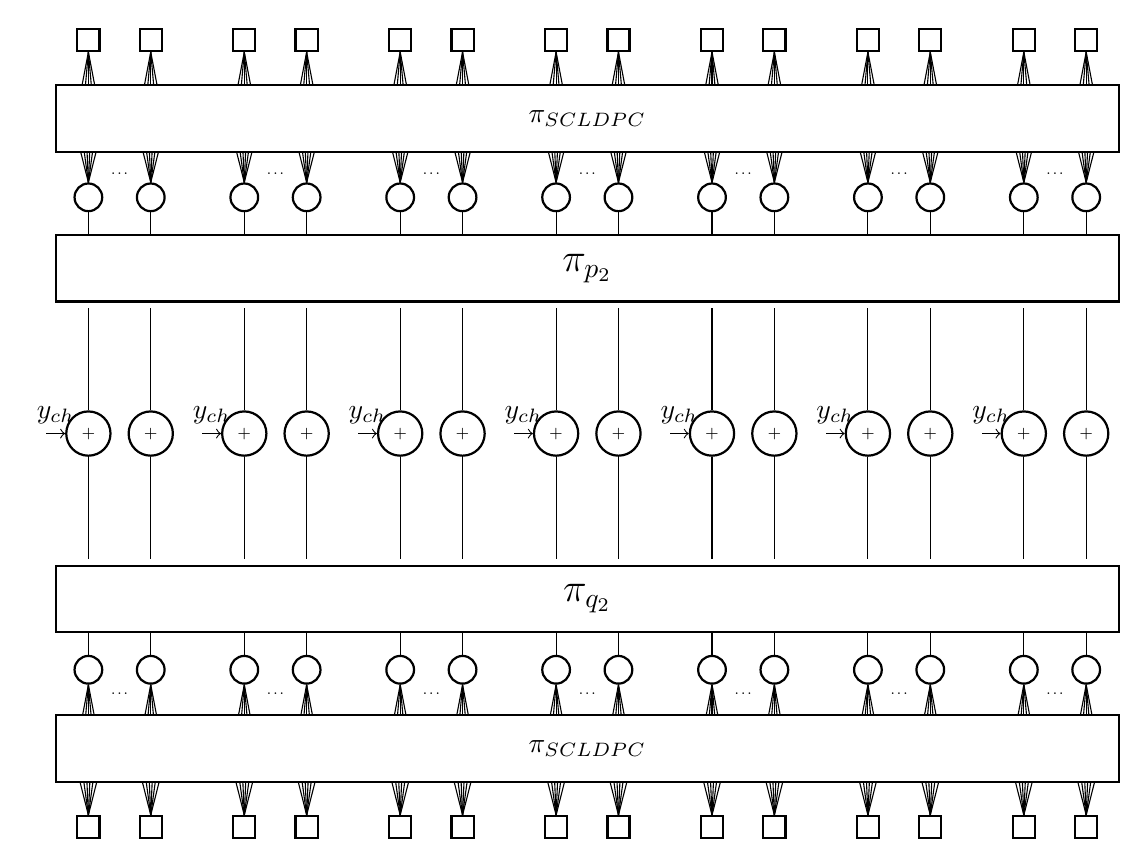
\begin{tikzpicture}[
  xscale=0.33,yscale=1,
  bitnode/.style={circle,minimum size=10pt,thick,draw=black,fill=white},
  bitnodeblack/.style={circle,minimum size=10pt,thick,draw=black,fill=white},
  bitnodewhite/.style={circle,minimum size=10pt,thick,draw=white,fill=gray},
  bitnode2/.style={circle,minimum size=10pt,thick,draw=black,fill=gray},
  bitnode2black/.style={circle,minimum size=10pt,thick,draw=black,fill=gray},
  bitnode2white/.style={circle,minimum size=10pt,thick,draw=white,fill=white},
  checknode/.style={rectangle,minimum size=8pt,thick,draw=black,fill=white},
  checknodeblack/.style={rectangle,minimum size=8pt,thick,draw=black,fill=white},
  checknodewhite/.style={rectangle,minimum size=8pt,thick,draw=white,fill=white},
  permnode/.style={rectangle,very thin,minimum width=30pt,minimum height=18pt,fill=white,draw=black},
  permnodeblack/.style={rectangle,very thin,minimum width=30pt,minimum height=18pt,fill=white,draw=black},
  permnodewhite/.style={rectangle,very thin,minimum width=30pt,minimum height=18pt,fill=white,draw=white},
  permedge/.style={black!65},
  permedgeblack/.style={black!65},
  permedgewhite/.style={white},
  ]

  \def \cndist {1.2}
  \def \vndist {1.2}
  \def \ccndist {1.2}
  \def \vvny {2.75}
  \def \cny {3}
  \def \vny {1}
  \def \vnya {-2}
  \def \vnyb {-5}
  \def \ccny {-7}
    \def \ext{1.3}
      \def \exta {1}
  \def \midx   {0.5}
  
    \tikzstyle{bigPerm}= [rectangle, draw, thick, minimum width=320*\vndist, minimum height=20*\vndist,fill=white, draw=black]
    
\def\ldgcol{black}
\def\ldpcol{black}
\def\seqa{black}
\def\seqb{black}
    \foreach \x/\i in {0/1,6/2,12/3,18/4,24/5,30/6,36/7} {

      \node[bitnode\seqa] (v1\i) at (\x-\vndist, \vny) {};
      \node[bitnode\seqa] (v2\i) at (\x+\vndist, \vny) {};
      \node at (\x,\vny+0.3) {\tiny{$...$}};
% Edges- LDPC bits to top
      \draw[\seqa] (v1\i.north) -- +(52.5:1);
      \draw[\seqa] (v1\i.north) -- +(67.5:1);
      \draw[\seqa] (v1\i.north) -- +(82.5:1);
      \draw[\seqa] (v1\i.north) -- +(97.5:1);
      \draw[\seqa] (v1\i.north) -- +(112.5:1);
      \draw[\seqa] (v1\i.north) -- +(127.5:1);

      \draw[\seqa] (v2\i.north) -- +(52.5:1);
      \draw[\seqa] (v2\i.north) -- +(67.5:1);
      \draw[\seqa] (v2\i.north) -- +(82.5:1);
      \draw[\seqa] (v2\i.north) -- +(97.5:1);
      \draw[\seqa] (v2\i.north) -- +(112.5:1);
      \draw[\seqa] (v2\i.north) -- +(127.5:1);


     \node[bitnode\seqb] (v3\i) at (\x-\vndist, \vnyb) {};
     \node[bitnode\seqb] (v4\i) at (\x+\vndist, \vnyb) {};
     \node at (\x,\vnyb-0.3) {\tiny{$...$}};
     
% Edges- LDPC bits to bottom
      \draw[\seqb] (v3\i.south) -- +(240:1);
      \draw[\seqb] (v3\i.south) -- +(255:1);
      \draw[\seqb] (v3\i.south) -- +(270:1);
      \draw[\seqb] (v3\i.south) -- +(285:1);
      \draw[\seqb] (v3\i.south) -- +(300:1);

      \draw[\seqb] (v4\i.south) -- +(240:1);
      \draw[\seqb] (v4\i.south) -- +(255:1);
      \draw[\seqb] (v4\i.south) -- +(270:1);
      \draw[\seqb] (v4\i.south) -- +(285:1);
      \draw[\seqb] (v4\i.south) -- +(300:1);

% Middle bits= Actual GMAC Code bits
    \node[bitnode] (v5\i) at (\x-\vndist, \vnya) {\tiny $+$};
    \node[bitnode] (v6\i) at (\x+\vndist, \vnya) {\tiny $+$};
     

    \draw (v1\i.south) -- +(270:\exta);      \draw (v2\i.south) -- +(270:\exta);    
    \draw (v3\i.north) -- +(90:\exta);        \draw (v4\i.north) -- +(90:\exta);

    \draw (v5\i.north)-- +(90:\ext);       \draw (v6\i.north)-- +(90:\ext);
    \draw (v5\i.south) -- +(270:\ext);    \draw (v6\i.south) -- +(270:\ext);

    \draw[<-] (v5\i.west) -- node[midway, above]{$y_{\text{ch}}$} +(-0.6*\vndist,0);

% Top Checks
 \node[checknode\ldgcol] (c1\i) at (\x-\cndist, \cny) {};
  \node[checknode\ldgcol] (c2\i) at (\x+\cndist, \cny) {};

% Top check to bottom
      \draw[\ldgcol] (c1\i.south) -- +(240:1);
      \draw[\ldgcol] (c1\i.south) -- +(255:1);
      \draw[\ldgcol] (c1\i.south) -- +(270:1);
      \draw[\ldgcol] (c1\i.south) -- +(285:1);
      \draw[\ldgcol] (c1\i.south) -- +(300:1);

      \draw[\ldgcol] (c2\i.south) -- +(240:1);
      \draw[\ldgcol] (c2\i.south) -- +(255:1);
      \draw[\ldgcol] (c2\i.south) -- +(270:1);
      \draw[\ldgcol] (c2\i.south) -- +(285:1);
      \draw[\ldgcol] (c2\i.south) -- +(300:1);

  
%Bottom Checks  
      \node[checknode\ldpcol] (cc1\i) at (\x-\ccndist, \ccny) {};
      \node[checknode\ldpcol] (cc2\i) at (\x+\ccndist, \ccny) {};
      
% Bottom checks to top
      \draw[\ldpcol] (cc1\i.north) -- +(52.5:1);
      \draw[\ldpcol] (cc1\i.north) -- +(67.5:1);
      \draw[\ldpcol] (cc1\i.north) -- +(82.5:1);
      \draw[\ldpcol] (cc1\i.north) -- +(97.5:1);
      \draw[\ldpcol] (cc1\i.north) -- +(112.5:1);
      \draw[\ldpcol] (cc1\i.north) -- +(127.5:1);

      \draw[\ldpcol] (cc2\i.north) -- +(52.5:1);
      \draw[\ldpcol] (cc2\i.north) -- +(67.5:1);
      \draw[\ldpcol] (cc2\i.north) -- +(82.5:1);
      \draw[\ldpcol] (cc2\i.north) -- +(97.5:1);
      \draw[\ldpcol] (cc2\i.north) -- +(112.5:1);
      \draw[\ldpcol] (cc2\i.north) -- +(127.5:1);

      \node[\ldpcol] at (\x,-5.7) {\tiny{$...$}};
      \node[\ldgcol] at (\x,1.7) {\tiny{$...$}};

}

  \node[bigPerm] (perm1_node) at (18,0.5*\vny+0.5*\cny) {\normalsize $\pi_{\text{SCLDPC}}$};    
  \node[bigPerm] (perm2_node) at (18,0.5*\vnyb+0.5*\ccny) {\normalsize $\pi_{\text{SCLDPC}}$};    
  
  \node[bigPerm] (perm3_node) at (18,0.7*\vny+0.3*\vnya) {\Large $\pi_{p_2}$};    
  \node[bigPerm] (perm4_node) at (18,0.3*\vnya+0.7*\vnyb) {\Large $\pi_{q_2}$};    
   
\end{tikzpicture}}
    \caption{Schematic showing the joint Tanner graph, of the channel coding component, for two users with message indices $w_1$ and $w_2$. In the SC-LDPC code $\pi_{\text{SCLDPC}}$ refers to a random permutation of the edge connections from  check nodes to bit nodes. For more details refer to \cite{kudekar2011threshold}. We introduce multiple access (MAC) node denoting the sum over the multiple access channel. For e.g., $k$-th MAC node is represented by $\vec{\mathrm{y}}_j^{\mathrm{c}}[k]=\sum_{i\in\{1,2\}}\cv_{w_i^{\mathrm{c}}}[\pi^k_{\tau_{w_i^\mathrm{p}}}]+\zv_{j}[k]$.}
	\label{fig:decodergraph}
\end{figure}

Given the received signal $\vec{\mathrm{y}}_j^{\mathrm{c}}$ the joint BP decoder proceeds iteratively in a similar manner to that of a single user AWGN channel decoding apart from an extra step of messages being sent to and received from the MAC node in each iteration. We use the following notation for the messages passed in the joint BP decoder:
\begin{itemize}
\item $u^{1}_{i,\text{MAC}},u^{1}_{i,j}$: messages passed from $i$-th bit node of user $1$ to the corresponding MAC node and  SCLDPC check node $j$ respectively
\item $v^{1}_{j,i}$: message passed from SCLDPC check node $j$ to bit node $i$ of user $1$
\item $v^{1}_{\text{MAC},i}$: message passed to $i^{\text{th}}$ bit node from corresponding MAC node of user $1$.
\end{itemize}
The messages for user $2$ are defined similarly. Refer to Fig. \ref{fig:BP_computationgraph} for a graphical representation of the messages. The message passing rules in the joint message passing decoder can be summarized as following.

bit node:
\begin{align*}
u^{1}_{i,j}&=v^{1}_{\text{MAC},i}+ \sum_{j'\neq j,j'\in \mathcal{N}(i)} v^{1}_{j',i}\\
u^{1}_{i,\text{MAC}}&=\sum_{j\in \mathcal{N}(i)} v^{1}_{j,i}
\end{align*}
SCLDPC check node:
\begin{align*}
v^{1}_{j,i}&=2~\tanh^{-1}\left( \prod_{i'\neq i} \tanh\left(\frac{u^{1}_{i',j}}{2}\right)\right).
\end{align*}
MAC node:
\begin{align}
v^{1}_{\text{MAC},i}&=h(u^{2}_{i,\text{MAC}},y_{i,\text{ch}})\label{Eqn:MACnodeBP} \\
v^{2}_{i,\text{MAC}}&=h(u^{1}_{i,\text{MAC}},y_{i,\text{ch}}) ~~~\text{ where}\notag\\
h(l,y)&=\log \frac{1+e^{l}e^{2(y-1)/\sigma^2}}{e^{l}+e^{-2(y+1)/\sigma^2}}.\notag
\end{align}
The function $h(l,y|\sigma^2)$ can be seen as the log-likelihood of variable $x_2$ when $y=x_1+x_2+z$, $x_1,x_2\in\{-1,+1\}$ when the log-likelihood ratio of variable $x_1$ is known to be $l$ and $z\sim \mc{N}(0,\sigma^2)$.
\begin{figure}[!ht]
  \centering
  \resizebox{0.75\textwidth}{!}{\begin{tikzpicture}
\def \depth{1.5}; %vertical gap between nodes/levels
\def \xgap{2.8}
\def \gap{0.6}; %Horizontal gap between nodes
\def \gapA{0.3}; %Encoder Width
\def \textoffs{0.24}; %Offset for writing text above a node
\def\nodewidth{0.5};
\tikzstyle{bitwhite} = [circle, draw, thick, fill=white, radius=0.5*\nodewidth]
\tikzstyle{bitshaded} = [circle, draw, thick, fill=gray, radius=0.5*\nodewidth]
\tikzstyle{checkwhite} = [rectangle, draw, thick, fill=white,minimum height=\nodewidth, minimum width=\nodewidth]
\tikzstyle{checkshaded} = [rectangle, draw, thick, fill=gray,minimum height=\nodewidth, minimum width=\nodewidth]
                          
\def \fsize{\footnotesize}; %Defining a generic font size to be adjusted depending on the scaling
\def \fsizea{\tiny}; %Defining a generic font size to be adjusted depending on the scaling
\def \dotsize{\Huge}; %Defining a generic font size to be adjusted depending on the scaling

%%---------------------- Graph 1---------------------------------------------------------------------------
\node [bitshaded](b1) at (0,0) {\fsizea $i$} ;
\node [bitwhite,radius=0.8*\nodewidth](bMAC) at (0,1) {\fsize $+$} ;
\draw[thick,decoration={markings,mark=at position 0.5 with {\arrow{>}}},postaction={decorate}] (b1.north) -- node[midway,left]{{\fsize $u_{i,\text{MAC}}$}} node[midway,right] {\fsize $=\sum\limits_{j=1}^{3}v_{j,i}$} (bMAC.south);

\foreach \i in {1,2,3}
{
\path (b1) -- +(180+\i*45:\depth) node[checkwhite] (c1\i) {\fsize $\i$};
\begin{scope}[decoration={ markings,    mark=at position 0.5 with {\arrow{>}}} ] 
\draw[postaction=decorate] (c1\i.north) -- node[pos=0.3,left]{{\fsize $v_{\i,i}$}} (b1);
\end{scope}
}

%%---------------------- Graph 2---------------------------------------------------------------------------
\node [bitshaded,radius=0.5*\nodewidth](bMAC2) at (\xgap,0) {\fsize $+$} ;
\node [bitwhite](b2) at (\xgap,1) {\fsizea $i$} ;
%\node () at (b2.east) {\fsizea User 2} ;
\draw[decoration={markings,mark=at position 0.5 with {\arrow{>}}},postaction={decorate}] (b2.south) -- node[midway,left]{{\fsize $u^{2}_{i,\text{MAC}}$}} (bMAC2.north);
\draw[decoration={markings,mark=at position 0.5 with {\arrow{<}}},postaction={decorate}] (bMAC2.west) -- node[midway,below]{{\fsize $y_{i,\text{ch}}$}} +(-0.25*\xgap,0);


\path (bMAC2) -- +(180+90:\depth) node[bitwhite] (b21) {\fsizea $i$};
\draw[thick,decoration={ markings, mark=at position 0.5 with {\arrow{<}}}, postaction=decorate] (b21.north) -- node[midway,left]{{\fsize $v^{1}_{\text{MAC},i}$}} (bMAC2);


%%---------------------- Graph 3---------------------------------------------------------------------------
\node [bitshaded](b3) at (2*\xgap,0) {\fsizea $i$} ;
\node [bitwhite,radius=0.8*\nodewidth](bMAC3) at (2*\xgap,1) {\fsize $+$} ;
\draw[decoration={markings,mark=at position 0.5 with {\arrow{<}}},postaction={decorate}] (b3.north) -- node[midway,left]{{\fsize $v_{\text{MAC},i}$}} (bMAC3.south);

\foreach \i in {1,2,3}
{
\path (b3) -- +(180+\i*45:\depth) node[checkwhite] (c3\i) {\fsize $\i$};
}
\foreach \i in {1,2}
{
\draw[decoration={ markings, mark=at position 0.5 with {\arrow{>}}}, postaction=decorate] (c3\i.north) -- node[pos=0.3,left]{{\fsize $v_{\i,i}$}} (b3.south);
}
\draw[thick,decoration={ markings, mark=at position 0.6 with {\arrow{<}}}, postaction=decorate] (c33.north) -- node[midway,right]{{\fsize $u_{i,3}=v_{\text{MAC},i}+\sum\limits_{j=1}^{2}v_{j,i}$}} (b3.south);

\end{tikzpicture}}
  \caption{ Message passing rules at individual nodes on the joint Tanner graph of two users. The message passing rules at the check nodes of the SCLDPC code are identical to the single user channel coding case.}
  \label{fig:BP_computationgraph}
\end{figure}


\subsection{Decoding process across sub-blocks - SIC}
For any sub-block $j$, if $\hat{R}_{j}<=T$ the $T$-user GMAC decoder within the sub-block, described in the previous sub-section, outputs the set of messages transmitted during the $j$-th sub-block. Given the decoded set of messages $\{w_i, i \in \mc{N}_j\}$ for sub-block $j$ and that the preamble collision detector output is negative, for each decoded message $w_i$:
\begin{itemize}
\item the sub-blocks where the codeword is repeated can be obtained using the function $g(w_i)$,
% For each decoded message in sub-block $j$,
\item  the codeword corresponding to message $w_i$ is subtracted or `peeled off' from the received signal in the corresponding repeated sub-blocks and
\item  in each of the repeated sub-blocks, the estimate $\hat{R}_k$ ($k$ being the sub-block) is updated (reduced by one) to account for the subtraction of one interfering codeword.
\end{itemize} 
The above process is repeated until either all the $\Ka$ messages are decoded or no sub-blocks with less than $T$ codewords remain. The above described iterative decoding process is known in the literature as successive interference cancellation (SIC). \\

\section{Choice of parameters and analysis}

In this section we analyze the performance of different components of the proposed scheme and the effect each of them has on the overall performance. At $j$-th sub-block where $R_j\leq T$ let us define the following error events:
%As described in Sec. \ref{Sec:SystemModel} let $\epsilon$ be the maximum per user error probability i.e. we are interested in decoding on an average $(1-\epsilon)$ fraction of the $\Ka$ active users successfully.
\begin{itemize}
\item $\mc{E}_{\mathrm{p}j}:$ Given there is no preamble collision, let $\mc{E}_{\mathrm{p}j}$ be the event that the output of the compressed sensing decoder is incorrect i.e., $\widehat{\mc{W}}_j^{\mathrm{p}}\neq \mc{W}_j^{\mathrm{p}}$. The event $\mc{E}_{\mathrm{p}}$ is defined for the worst case $R_j=T$
\item $\mc{E}_{\mathrm{e}j}:$ Let $\mc{E}_{\mathrm{e}j}$ be the event that the error energy test makes an error. With the following notations:
\begin{itemize}
\item  Given that there is no preamble collision and the compressed sensing decoder is correct let $\mc{E}_{\mathrm{e}j}^{0}$ be the event the error energy test detects a preamble collision and 
\item let $\mc{E}_{\mathrm{e}j}^1$ be the event there exists a collision but the energy test fails to detect the preamble collision 
\end{itemize}
we can see that $\mc{E}_{\mathrm{e}j}=\mc{E}_{\mathrm{e}j}^0 \cup \mc{E}_{\mathrm{e}j}^1$.
\item $ \mc{E}_{\mathrm{c}j}:$ Given there is no preamble collision and that the preamble message indices are decoded successfully, let $\mc{E}_{\mathrm{c}j}$ be the event that the channel decoder fails to recover all the channel coding message indices correctly. The event $\mc{E}_{\mathrm{c}}$ is defined for the worst case, when $R_j=T$
\item $\mc{E}_{\text{SIC}}:$ Let $\mc{E}_{\text{SIC}}$ be the event that a random user is not recovered by the SIC decoding process
\end{itemize}
We observe that the overall decoding process within a given sub-block $j$ making an error is a disjoint union of the above described events i.e., 
\begin{align*}
\mc{E}_j&=\mc{E}_{\mathrm{p}j}\cup\mc{E}^0_{\mathrm{e}j}\cup \mc{E}_{\mathrm{c}j} \cup \mc{E}^1_{\mathrm{e}j}\\
&=\mc{E}_{\mathrm{p}j}\cup\mc{E}_{\mathrm{e}j}\cup \mc{E}_{\mathrm{c}j}.
\end{align*}
The per user error probability $P_e$, which is equivalent to $\Pr\left(\mc{E}_{\text{SIC}}\right)$, can be bounded as following:
\begin{align}
P_e=\Pr\left(\mc{E}_{\text{SIC}}\right) &\leq \Pr\left(\mc{E}_{\text{SIC}}| ~(\bigcup_{j}\mc{E}_j)^c\right)+ \Pr\left(\bigcup_{j}\mc{E}_j\right)\notag\\
&\leq \Pr\left(\mc{E}_{\text{SIC}}|~\bigcap_{j}\mc{E}_j^c\right)+ \Pr\left(\bigcup_{j}\mc{E}_{\mathrm{p}j}\cup \mc{E}_{\mathrm{e}j}\cup \mc{E}_{\mathrm{c}j}\right)\notag\\
&\leq\Pr\left(\mc{E}^{'}_{\text{SIC}}\right)+\sum_{j} (\Pr (\mc{E}_{\mathrm{p}j})+\Pr (\mc{E}_{\mathrm{e}j}) \Pr (\mc{E}_{\mathrm{c}j}))\notag\\
&\leq\Pr\left(\mc{E}^{'}_{\text{SIC}}\right)+V\left(\Pr(\mc{E}_{\mathrm{p}})+\Pr (\mc{E}_{\mathrm{e}})+\Pr(\mc{E}_{\mathrm{c}}) \right) \label{eqn:errPrb_split}
\end{align}
where $\mc{E}^{'}_{\text{SIC}}$ is the event of a user not being recovered under the SIC decoder assuming that the compressed sensing decoder, collision detector and the channel decoder do not make any errors. The precise characterization of this decoding process, referred to as simplified SIC, that can be used to evaluate $\Pr\left(\mc{E}^{'}_{\text{SIC}}\right)$ is given in Def.~\ref{def:simple_SIC}. The multiplicative factor $V$ in Eqn. \eqref{eqn:errPrb_split} union bounds the total number of instances(sub-blocks) compressed sensing decoder, the collision detector or the channel decoder can commit an error.

\begin{definition}[Simplified SIC decoder]
\label{def:simple_SIC}
We define simplified SIC decoder as an iterative decoding process on a bipartite graph with two types of nodes, variable and slot. Consider a graph wherein the users represent variable nodes and sub-blocks represent slot nodes. Each variable node is associated with a unique preamble message index chosen independently and uniformly at random from $[\Mp]$. Simplified SIC decoder proceeds iteratively on the bipartite graph in which at any slot node if the number of variable nodes connected is less than or equal to $T$:
\begin{itemize}
\item  if there is no preamble collision between the connected variable nodes, then the respective variable nodes are assumed to have been decoded successfully. All the connected variable nodes and their edges will be peeled off from the graph
\item if there is a preamble collision, then the slot node is simply ignored in this iteration.
\end{itemize}  
\end{definition}
 The idea behind the simplification is that the sub-blocks in which there is a preamble collision need not necessarily result in an error, but they can be resolved in future iterations when one of the colliding users has been decoded and peeled off from the sub-block.

%where we refer to the SIC process under the assumption that the preamble collision, CS decoder error and the MAC channel decoder error do not occur in any of the slots as $T$-peeling or ideal SIC process. In other words $T$-peeling is an iterative process in which at any slot if there are less than or equal to $T$-users connected we assume those $T$-users are decoded and their contributions are subtracted off (peeled off from the slot nodes) from the other slots in which these users have transmitted. Thus the event $\mc{E}_{\text{SIC}}$ conditioned on $\cap_{i,j}\mc{E}^c_{ij}$ is equivalent to the event a random user is not recovered under the $T$-peeling process which is denoted $\mc{E}_{T\text{-peeling}}$. The multiplicative factor $V$ in the upper bound of $P_e$ in Eqn. \eqref{eqn:errPrb_split} union bounds the total number of instances(slots) a preamble collision ($\mc{E}_1$) or a compressed sensing decoder error ($\mc{E}_2$) or a MAC channel decoder error ($\mc{E}_3$) can occur.

%$\mc{E}_4|\epsilon_0$ is the event that the SIC process does not recover atleast $(1-\epsilon_0)$ fraction of the all the users' messages.
%Let theFor a fixed number of active users $K_a$, maximum number of users jointly decoded at a sub-block $T$, total number of channel uses $n$ and the number of bits transmitted by each user $B$, let $P_e$ denote the probability that a user is not decoded successfully. Then $P_e$ can be upper bounded by  %of the error event where atleast $(1-\epsilon)$ fraction of the users are not decoded successfully. A standard union bound on the probability of error $P_e$ is given by
%We denote $\mc{E}_1$ to be the event where at least two messages get hashed to the same shift, i.e., $\exists i,j$ s.t. $\tau_{w_i} = \tau_{w_j}$. According to our decoding process, since we can detect hash collisions with high probability, we simply use $V(1+P\left(\mc{E}_1\right)$ slots and the slots that are determined to contain hash collisions are not used for the $T$-user decoding.


\subsection{Compressed sensing problem and design choices}
In this section we discuss the choice of parameters $T,\Bc$ (or equivalently $\Mp$), sensing matrix $\mathbf{A}$ and analyze the performance of the preamble component for various such  choices under the correlation and list decoders described in Sec.\ref{subsubsec:decoder_subblock}. 

We consider two options for the choice of sensing matrix: (i) random matrix with each entry chosen according to Rademacher distribution, referred to as \textit{random ensemble} and (ii) sensing matrix derived as a subset of a binary code with good minimum distance properties, referred to as \textit{binary ensemble}. 

\subsubsection*{random ensemble} 
For a given $\Np$ and $\Mp$ a sensing matrix $\mathbf{A}=[a_{ij}]_{i\in[\Np],j\in[\Mp]}$ from \emph{random} ensemble is obtained by choosing each $a_{ij}=\pm \sqrt{\Pp}$, independently, with equal probability.

\subsubsection*{binary ensemble} 
A sensing matrix from \emph{binary} ensemble is derived as a subset of a binary linear code with appropriate scaling and shifting. More precisely, for a given $\Np$ and $\Mp$, let $\mc{C}_{\text{bin}}$ be a subset of size $\Mp$, not necessarily a sub-code, of a binary linear code with block length $\Np$. Then the sensing matrix is obtained by $\mathbf{A}=\sqrt{\Pp}(1-2 \mc{C}_{\text{bin}})$. Also let the minimum and maximum Hamming distances between any two binary vectors in $\mc{C}_{\text{bin}}$ be represented by $\dmin$ and $\dmax$ respectively.

For the \emph{random} and \emph{binary} ensembles described above the following lemma gives the probability of error under correlation decoder for a given $T$ denoting the sparsity.
\begin{lemma}[Compressed sensing with correlation decoder]
\label{lem:errorprob_correlationdecoder}
Consider the $T$-sparse support recovery problem where let $\{1,2,\ldots,T\}$ be the set of sparse indices without loss of generality and $\yv$ be the preamble part of the received vector. The probability of error for the correlation decoder  %compressed sensing problem with the correlation decoder 
can then be bounded by
\begin{align}
\Pr(\mc{E}_{\mathrm{p}})&=1-\left(1-(\Mp-T)\Pr(\mc{E}_{\text{corr}})\right)^T \label{eqn:Pecorrdecoder}\\
%+ \left((1+\Pp)e^{-\Pp}\right)^{\Np/2}
&\leq T(\Mp-T)\Pr(\mc{E}_{\text{corr}})\notag,% +\left((1+\Pp)e^{-\Pp}\right)^{\Np/2}
\end{align}
where $\Pr(\mc{E}_{\text{corr}})$ denotes the the probability of the error event that the correlation $\langle \yv, \av_i\rangle \leq \langle \yv, \av_j\rangle $ for some $i\leq T$ and $j>T$. For the \emph{random} and \emph{binary} ensembles this can be upper bounded by 
%denotes the probability that the correlation of the received vector with one of the $T$ sparse vectors is smaller than with a randomly chosen non-sparse vector. 
\begin{align}
\text{random ensemble:}\qquad ~~&\Pr(\mc{E}_{\text{corr}})\leq \exp\left\lbrace\frac{-\Np\Pp}{2(2+(2T-1)\Pp)}\right\rbrace\label{eqn:Pecorr_random}\\
\text{binary ensemble:}\qquad ~~&\Pr(\mc{E}_{\text{corr}})\leq \exp\left\lbrace\frac{-\Pp\dmax (1-T(1-\dmin/\dmax))^2}{2}\right\rbrace.\label{eqn:Pecorr_binary}
\end{align}
\end{lemma}
\begin{proof}
We observe that the correlation decoder makes an error if there exists $i\leq T$ and $j>T$ such that $\langle \yv, \av_i\rangle \leq\langle \yv, \av_j\rangle $ the probability of which is given by the right hand side in Eqn. \eqref{eqn:Pecorrdecoder}. The analysis for the event $\mc{E}_{\text{corr}}$ and the bounds in Eqns. \eqref{eqn:Pecorr_random} and \eqref{eqn:Pecorr_binary} are provided in Appendix.~\ref{appendix:proof_errorprob_correlationdecoder}. 
\end{proof}
 For the random ensemble we observe from Equations. \eqref{eqn:Pecorrdecoder} and \eqref{eqn:Pecorr_random} that the error probability of correlation decoder decreases exponentially in the number of channel uses $\Np$. However, with respect to SNR $\Pp$, the rate of decay is very slow. In fact it converges to a positive value
\[
\Pr(\mc{E}_{\text{corr}})\rightarrow \exp\left\lbrace\frac{-\Np}{2(2T-1)}\right\rbrace.
\]
 If we consider the binary ensemble, the error probability of the overall decoder decays exponentially in both the channel uses $\Np$ and SNR $\Pp$ given that the subset $\mc{C}_{\text{bin}}$ has the following properties:
 \begin{itemize}
 \item The gap between minimum and maximum Hamming distances $\dmax-\dmin$ is small
 \item The minimum distance $\dmin$ is large. Note that this in conjunction with the above condition implies a large $\dmax$ which is necessary for a large exponent $\frac{-\Pp\dmax (1-T(1-\dmin/\dmax))^2}{2}$ %$\frac{-\Pp(\dmax-T(\dmax-\dmin))^2}{2(\Np-\dmax)}$.
 \end{itemize}
Based on the design objectives outlined above, we design a sensing matrix from the $\emph{binary ensemble}$ for a toy example with parameters $\Mp=512,\Np=63$.
\begin{example}[Sensing matrix from binary ensemble]
\label{ex:sensingmatrix_BCHsubset}
%Note that $\Mp=2^{\Bp}=512$ is the size of the sensing matrix $\mathbf{A}$. 
Let binary code $\mc{C}_{\text{BCH}}$ be the BCH$(63,10)$ code of size $1024$. We obtain a subset of $\mc{C}_{\text{BCH}}$ of size $M_\mathrm{p}$ by the following decomposition
\[
\mc{C}_{\text{BCH}}=\mc{C}_0\cup \mc{C}_1 ~~\text{ such that } c\in \mc{C}_1 \iff \bar{c}\in\mc{C}_0,
\]
where $\bar{c}=\mathbf{1}\oplus c$ i.e., the one's complement of $c$. We choose the sensing matrix of size $\Np \times \Mp=63\times 512$ as $\mathbf{A}=[\av_1,\av_2,\ldots,\av_{M_\mathrm{p}}],$ where $\av_i=\sqrt{\Pp}(1-2\cv_i), \cv_i\in\mc{C}_1$, i.e., $a_{ij}\in\{-\sqrt{\Pp},\sqrt{\Pp}\} \forall i,j$. This specific decomposition allows us to maintain the minimum distance $\dmin=28$ identical to the original code $\mc{C}_{\text{BCH}}$ while reducing the maximum distance for the subset $\mc{C}_1$ to $\dmax=36$ from $63$ of the original code.
\end{example}
 In Fig.~\ref{fig:cscomparison} we present the error performance results for the sensing matrix in Example~\ref{ex:sensingmatrix_BCHsubset} under correlation decoder and compare with the performance of a sensing matrix from the random ensemble. It can be clearly seen that correlation decoder is sub-optimal. Therefore we also present the performance of both the ensembles under the list decoder. Although the list decoder is difficult to analyze primarily due to the LASSO and constrained least squares optimization algorithm components, it can be seen from Fig.~\ref{fig:cscomparison} that the list decoder has superior performance when compared to the correlation decoder via numerical simulations.

\begin{figure}[!ht]
  \centering
  \resizebox{0.75\textwidth}{!}{% This file was created by matlab2tikz v0.4.7 running on MATLAB 7.14.
% Copyright (c) 2008--2014, Nico Schlömer <nico.schloemer@gmail.com>
% All rights reserved.
% Minimal pgfplots version: 1.3
% 
% The latest updates can be retrieved from
%   http://www.mathworks.com/matlabcentral/fileexchange/22022-matlab2tikz
% where you can also make suggestions and rate matlab2tikz.
% 
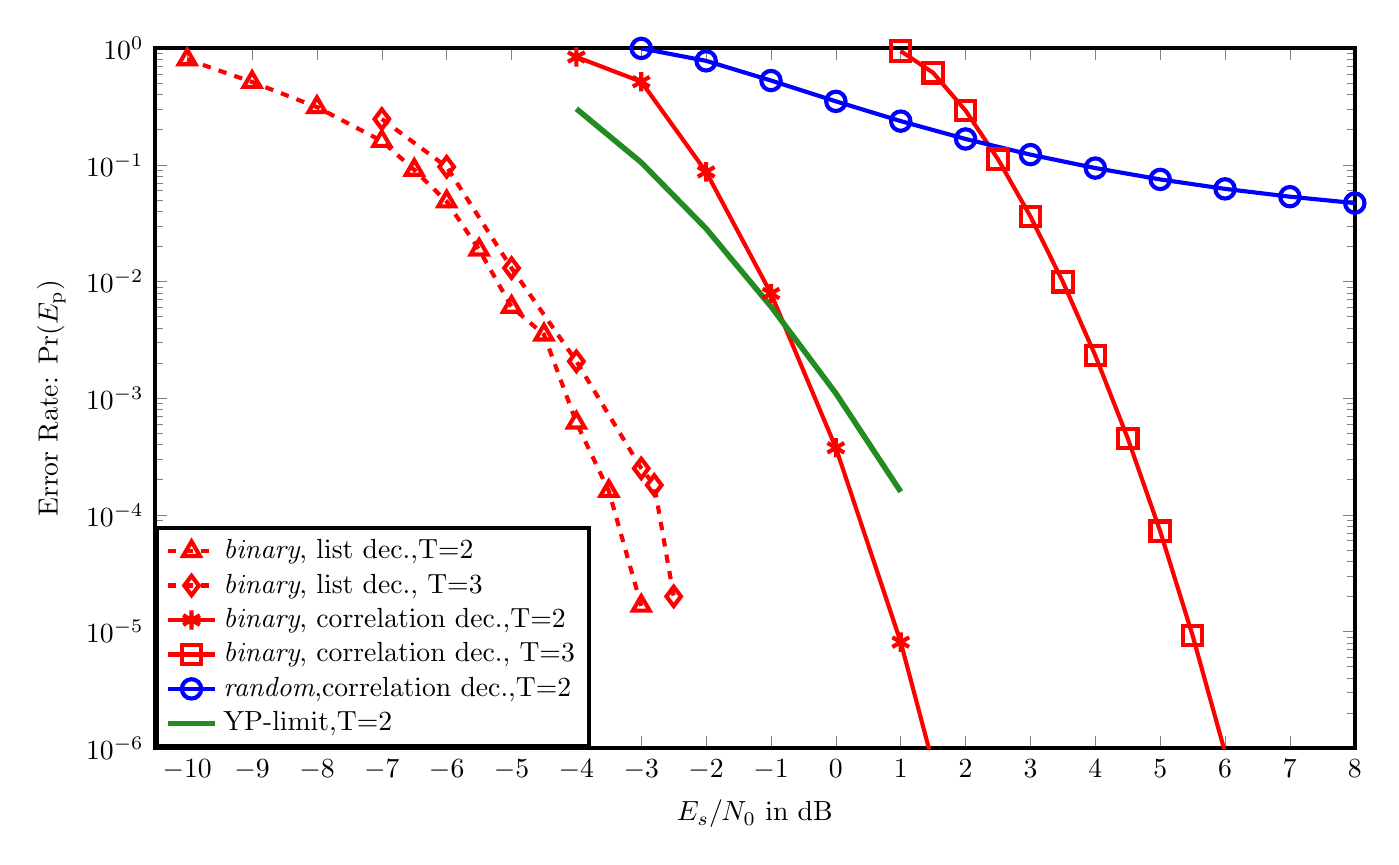
\begin{tikzpicture}

\begin{axis}[%
width=6in,
height=3.5in,
scale only axis,
xmin=-10.5,
xmax=8,
xtick={-10,-9,...,8},
xlabel={$E_s/N_0$ in dB},
ymode=log,
ymin=1e-6,
ymax=1,
ylabel={Error Rate: $\Pr(\mc{E}_{\mathrm{p}})$},
line width=1.5pt,
mark size=3.5pt,
legend style={at={(0,0)},anchor=south west,draw=black,fill=white,legend cell align=left}
]

\addplot [color=red,dashed,mark=triangle,mark options={solid}]
  table[row sep=crcr]{
  -10.00 8.000000e-01 \\
-9.00 5.128205e-01 \\
-8.00 3.125000e-01 \\
-7.00 1.600000e-01 \\
-6.50 9.049774e-02 \\
-6.00 4.842615e-02 \\
-5.50 1.876173e-02 \\
-5.00 6.064281e-03 \\
-4.50 3.506926e-03 \\
-4.00 6.165798e-04 \\
-3.5 1.60e-4\\
-3   1.66e-5\\
};
\addlegendentry{\emph{binary}, list dec.,T=2};

\addplot [color=red,dashed,mark=diamond,mark options={solid}]
  table[row sep=crcr]{
-7.00 2.469136e-01 \\
-6.00 9.615385e-02 \\
-5.00 1.302932e-02 \\
-4.00 2.067825e-03 \\
-3.00  2.50e-4\\
-2.8    1.80e-4\\
-2.50  2.00e-5\\
};
\addlegendentry{\emph{binary}, list dec., T=3};

%--------------Binary Correlation---------------------------------------
\addplot [color=red,solid,mark=asterisk]
  table[row sep=crcr]{-4	0.839938973915005\\
-3	0.515644197871796\\
-2	0.0869483964858722\\
-1	0.00788931487190525\\
0	0.000375462939704696\\
1	8.10369067605343e-06\\
2	6.47753143345753e-08\\
3	1.4828516192722e-10\\
4	7.03881397612349e-14\\
};
\addlegendentry{\emph{binary}, correlation dec.,T=2};


\addplot [color=red,solid,mark=square]
  table[row sep=crcr]{
1.00 9.441071e-01 \\
1.50 6.145469e-01 \\
2.00 2.916389e-01 \\
2.50 1.116871e-01 \\
3.00 3.606143e-02 \\
3.50 9.930853e-03 \\
4.00 2.319413e-03 \\
4.50 4.526161e-04 \\
5.00 7.231748e-05 \\
5.50 9.236722e-06 \\
6.00 9.177669e-07 \\
6.50 6.879983e-08 \\
7.00 3.759705e-09 \\
7.50 1.441054e-10 \\
8.00 3.710032e-12 \\
};
\addlegendentry{\emph{binary}, correlation dec., T=3};

%--------------Random Correlation---------------------------------------
\addplot [color=blue,solid,mark=o]
table[row sep=crcr]{
-3	0.995230206114719\\
-2	0.778551914311517\\
-1	0.527915283916314\\
0	0.350147600825551\\
1	0.237010766866583\\
2	0.166567660059161\\
3	0.122277177522\\
4	0.0937964411765719\\
5	0.0749838370997399\\
6	0.0622164196527422\\
7	0.0533299595443338\\
8	0.0470037470917604\\
9	0.0424113405143324\\
10	0.0390218393634084\\
11	0.0364852502123492\\
12	0.0345650780260551\\
13	0.0330978144887919\\
14	0.0319680291755858\\
15	0.0310926979824901\\
};
\addlegendentry{\emph{random},correlation dec.,T=2};

%-----------------------------------------------------------------
\addplot [color=ForestGreen,solid,line width=2pt]
table[row sep=crcr]{
-4  0.3022\\
-3	 0.1048\\
-2	 0.0284\\
-1	0.0061\\
0	0.0011\\
1 1.5778e-04\\
};
\addlegendentry{YP-limit,T=2};



\end{axis}
\end{tikzpicture}%}
  \caption{For $\Np=63, \Mp=512$ we compare the performance of the \emph{binary} and \emph{random} ensembles under list and correlation decoders for $T=\{2,3\}$. The sensing matrix for binary ensemble is given in Ex.~\ref{ex:sensingmatrix_BCHsubset}. For the correlation decoder we simply use the performance bounds given in Lemma.~\ref{lem:errorprob_correlationdecoder} whereas for the list decoder we perform numerical simulations using list decoder where we use non-negative least squares for the first component of the decoder.}
  \label{fig:cscomparison}
\end{figure}
%\input{compressed_sensing.tex}

\subsection{Energy test}
In this section we analyze the the performance of the error energy test component.
\begin{lemma}
\label{lem:energytest_overallerror}
The probability of the event that the energy test makes an error can be bounded by
\[
\Pr(\mc{E}_{\mathrm{e}})\leq  \left((1+\Pp)e^{-\Pp}\right)^{\Np/2} + \frac{T(T-1)}{2M_\mathrm{p}} \Pr\left( \frac{1}{\Np}||\av_i+\av_j+\zv||^2\leq (1+\Pp)\right),
\]
where $i,j$ are distinct indices chosen randomly from the set $[\Mp]$.
\end{lemma}
\begin{proof}
If we let $\Pr(\mc{E}_{\text{coll}})$ be the event that there is a preamble collision, then
\begin{align*}
\Pr(\mc{E}_{\mathrm{e}})&=\Pr(\mc{E}_{\mathrm{e}},\mc{E}_{\text{coll}}^c)+\Pr(\mc{E}_{\mathrm{e}},\mc{E}_{\text{coll}})\\
&\leq \Pr(\mc{E}_{\mathrm{e}}|\mc{E}_{\text{coll}}^c)+\Pr(\mc{E}_{\text{coll}})\Pr(\mc{E}_{\mathrm{e}}|\mc{E}_{\text{coll}})\\
&\stackrel{(a)}{=}\Pr(\mc{E}_{\mathrm{e}}^0)+\Pr(\mc{E}_{\text{coll}}) \Pr(\mc{E}_{\mathrm{e}}^1) 
\end{align*}
where substituting the results from Lemmas.~\ref{lem:energytest_fail}, \ref{lem:energytest_pass} and \ref{lem:hashCollision} in (a) completes the proof.
\end{proof}

\begin{lemma}
\label{lem:energytest_fail}
$\Pr(\mc{E}_{\mathrm{e}}^0)\leq \left((1+\Pp)e^{-\Pp}\right)^{\Np/2}$
\end{lemma}
\begin{proof}
Given there is no preamble collision and the compressed sensing decoder is successful, $\Pr(\mc{E}_{\mathrm{e}}^0)$ can be bounded as
\begin{align*}
\Pr(\mc{E}_{\mathrm{e}}^0)&=\Pr\left(\frac{1}{\Np}||\yv-\sum_{i\in\widehat{\mc{N}}_j}\av_i||^2 >1+\Pp\right)\\
&=\Pr\left(\frac{1}{\Np}||\zv||^2 >1+\Pp\right)
\end{align*}
the probability of which can be upper bounded using the tail bound of chi-squared distribution.
\end{proof}

\begin{corollary}
\label{lem:energytest_pass}
Let $i,j$ be distinct indices chosen randomly from the set $[\Mp]$, then
\[
\Pr(\mc{E}_{\mathrm{e}}^1)\leq \Pr\left( \frac{1}{\Np}||\av_i+\av_j+\zv||^2\leq 1+\Pp\right)
\]
\end{corollary}
\begin{proof}
%Given there is a preamble collision,
Let the set of $T$ preamble indices be $\mc{W}^{\mathrm{p}}$ and the output of the compressed sensing decoder be $\widehat{\mc{W}}^{\mathrm{p}}$.
 %outputs a set of $T$ distinct indices which let us denote by $\widehat{\mc{W}}^{\mathrm{p}}$, and hence makes an error.
%In case of preamble collision, the compressed sensing decoder makes an error.  there exists  the compressed sensing decoder makes an error Therefore without loss of generality let the set of $T$ preamble indices be $\mc{W}^{\mathrm{p}}=\{1,1,2,\ldots,T-1\}$ and the output of the compressed sensing decoder be $\widehat{\mc{W}}^{\mathrm{p}}$. 
\begin{align*}
\Pr(\mc{E}_{\mathrm{e}}^1)&=\Pr\left(\frac{1}{\Np}||\yv_j^{\mathrm{p}}-\sum_{i\in\widehat{\mc{W}}_j^{\mathrm{p}}}\av_i||^2 \leq (1+\Pp)\right)
\end{align*}
\begin{align*}
&=\Pr\left(\frac{1}{\Np}||\sum_{i\in\mc{W}_j^{\mathrm{p}}}\av_i-\sum_{i\in\widehat{\mc{W}}_j^{\mathrm{p}}}\av_i+\zv||^2 \leq (1+\Pp)\right)\\
&=\Pr\left(\frac{1}{\Np}||\sum_{i\in\mc{W}^{\mathrm{p}} \bigtriangleup\widehat{\mc{W}}^{\mathrm{p}} }\av_i +\zv||^2 \leq (1+\Pp)\right)\\
&\stackrel{(b)}{\leq}\Pr\left(\frac{1}{\Np}||\av_i +\av_j +\zv||^2 \leq (1+\Pp)\right)
\end{align*} 
where for ($b$) we recall that the compressed sensing decoder outputs $T$ distinct preamble indices whereas $\mc{W}^{\mathrm{p}}$ has atleast one repeating preamble index and thus $|\mc{W}^{\mathrm{p}} \bigtriangleup\widehat{\mc{W}}^{\mathrm{p}}|\geq 2$. 
\end{proof}

\begin{lemma}
$\Pr \left(\mc{E}_{\text{coll}}\right)\leq \frac{T(T-1)}{2M_\mathrm{p}}$.
\label{lem:hashCollision}
\end{lemma}
\begin{proof}
Let us consider the event $\mc{E}_{\text{coll}}^c$ where the $T$ users in the slot picked a unique preamble message index. Note that in total there are $M_\mathrm{p}$ possible preamble indices for each user.
\begin{align}
\Pr(\mc{E}_{\text{coll}}^c)&=\frac{M_\mathrm{p}(M_\mathrm{p}-1)\ldots(M_\mathrm{p}-(T-1))}{M_\mathrm{p}^{T}}\notag\\
\implies \Pr(\mc{E}_{\text{coll}})&=1-\prod_{i=0}^{T-1}(1-\frac{i}{M_\mathrm{p}})\notag\\
&\leq \frac{T(T-1)}{2M_\mathrm{p}}.\label{eqn:Hashcollision}
\end{align}
\end{proof}

\ifolder
\subsection{Preamble collision}
\begin{lemma}
$\Pr \left(\mc{E}_{1}\right)\approx \frac{T(T-1)}{2M_\mathrm{p}}$	
\label{lem:hashCollision}\\
\end{lemma}
\begin{proof}
Let us consider the event $\mc{E}_{1j}^c$ where the $R_j$ users in slot $j$ picked a unique preamble message index (or equivalently a unique permutation). Note that in total there are $M_\mathrm{p}$ possible preamble indices for each user.
\begin{align}
\Pr(\mc{E}_{1j}^c)&=\frac{M_\mathrm{p}(M_\mathrm{p}-1)\ldots(M_\mathrm{p}-(R_j-1))}{M_\mathrm{p}^{R_j}}\notag\\
\implies \Pr(\mc{E}_{1j})&=1-\prod_{i=0}^{R_j-1}(1-\frac{i}{M_\mathrm{p}})\notag\\
&\approx \frac{R_j(R_j-1)}{2M_\mathrm{p}}.\label{eqn:Hashcollision}
\end{align}
According to the encoding scheme each user chooses the slot randomly according to the message index and hence the degree distribution for the slots is non-uniform. But we observe that the CS and the channel decoders are run on a slot only when the remaining number of connections are estimated to be less than $T$ and hence we can approximate the number of connections to $T$ to get a uniform upper bound  across the slots. Substituting $T$ for $R_j$ in Eqn. \eqref{eqn:Hashcollision} completes the proof.
\end{proof}

\subsection{Compressed sensing problem and design choices}
Now we discuss our choice of parameters for $T, B_\mathrm{c}, B_\mathrm{p}$ and the sensing matrix $\mathbf{A}$. First let us start with the sensing matrix and the recovery of the sparse signal that aids in recovering the set of preamble message indices. In this chapter the typical values considered for $T$  are $\{2,4\}$. A low probability of error for event $\mc{E}_2$, for such low values of $T$, translates to  designing a sensing matrix $\mathbf{A}$ where we require: 
\begin{enumerate}
\item A large minimum distance in the Euclidean space between distinct $T$-sums of columns and 
\item a minimal number of $T$-sets of columns whose sum is identical.
\end{enumerate} 
Before we formalize the above mentioned notions, we would like to note that, for the choice of $\mathbf{A}$, we considered the superimposed codes proposed by authors Fan, Darnell and Honary for the multiaccess binary adder channel \cite{fan1995superimposed}. In this work the authors consider binary codes and show that every constant weight code with weight $w$ and maximum correlation $c$ corresponds to a subclass of disjunctive code of order $T<\frac{w}{c}$. In other words, for any $T<\frac{w}{c}$ sum of any $T$ codewords from this code results in a distinct output. Although the superimposed codes solve the second requirement we mentioned above they do not consider the first requirement i.e., the larger minimum distance of the resulting signal space of $T$-sums of codewords which is also critical to obtain a low probability of decoding error values. We defer the discussion of these results and our result relaxing the constraint of \textit{constant weight} to appendix.

In the following subsection we introduce lattice and derive upper bounds on $\Pr(\mc{E}_2)$ based on maximum-likelihood decoder for lattices.
% We consider superimposed codes for the multiaccess binary adder channel \cite{fan1995superimposed} for the choice of $\mathbf{A}$ which exactly fits our purpose. In this work authors Fan, Darnell and Honary consider binary codes for the multiple access real adder channel and show that every constant weight code with weight $w$ and maximum correlation $c$ corresponds to a subclass of disjunctive code of order $T<\frac{w}{c}$. In other words, for any $T<\frac{w}{c}$ sum of any $T$ codewords from this code results in a distinct output and thus this class of constant weight codes serve as a good choice for our sensing matrix $\mathbf{A}$. \\
\begin{definition}
A lattice $\Lambda$ in $n$-dimensional Euclidean space $\Lambda\subset \mathbb{R}^{n}$ can be defined as:
% is a discrete set of points in Euclidean space that form an additive group. More precisely an $m$-dimensional lattice $\Lmb^{(n)}\subset \R^{n}$ can be defined as:
\begin{equation}
\Lambda =\{\lambda\in\mathbb{R}^{n}:\lambda=\mathbf{G}\mathbf{u},\mathbf{u}\in \mathbb{Z}^{m}\}
\end{equation}
where $\mathbf{M}\in\mathbb{R}^{n \times m}$ is called the generator matrix of the lattice. We define the minimum distance $\dmin(\Lambda)$ of the lattice $\Lambda$ as 
\[
\dmin(\Lambda)\defeq \min_{\lambda_1, \lambda_2\in\Lambda } ||\lambda_1-\lambda_2||_2.
\]
\end{definition}

Let the set of codewords/columns of $\mbf{A}$ be denoted by $\mc{C}$ and $\mc{C}\subseteq \mc{C}_{\text{lin}}$ where $\mc{C}_{\text{lin}}$ is a binary linear code. We can then observe that the set of $T$-sums of codewords is a subset of lattice formed from $\mc{C}_{\text{lin}}$ ie..,
\begin{align*}
\sum_{j=1}^{T}\vec{a}_{i_j}&\in \Lambda ~~ i_j\in[1:M_\mathrm{p}]
\end{align*}
where $\Lambda =\{\mathbf{G}\mathbf{u},\mbf{u}\in \mbb{Z}^{m}\}, \mbf{G}$ is the generator matrix of the binary code $\mc{C}_{\text{lin}}$. Now that the connection between the $T$-sums of the binary code and the lattice in which they are contained in is established we formalize the two requirements on $\mbf{A}$ mentioned above.
%\begin{definition}
%For a given binary code $\mc{C}$ and fixed $T$, we define the parameter 
%\[
%\beta_T(\mc{C})\defeq |\{S:\exists S' \text{ s.t.} \sum_{i\in S}\vec{c}_i= \sum_{i\in S'}\vec{c}_i, |S|=|S'|=T,S\neq S'\}|,
%\]
%which counts the number of subsets of size $T$ whose sum is not unique in the set of $T$-sums of codewords from $\mc{C}$. The second requirement mentioned above translates to minimizing $\beta_T(\mc{C})$.
%\label{Def:disjunctive_parameter_Tsum}
%\end{definition}

%\begin{definition}
%For a given binary code $\mc{C}$ and fixed $T$, we define the minimum distance parameter
%\[
%\dmin(\mc{C},T)\defeq \min_{S\neq S',|S|=|S'|=T} ||\sum_{i\in S}\vec{a}_i-\sum_{i\in S'}\vec{a}_i||_2,
%\]
%which counts the minimum Euclidean distance between the $T$-sums of codewords. Note that $\beta_T(\mc{C})>0$ implies $\dmin(\mc{C},T)=0$ and $\beta_T(\mc{C})=0$ implies $\dmin(\mc{C},T)\geq \dmin(\Lambda)$.
%\label{Def:dmin_Tsum}
%\end{definition}

\begin{definition}
For a given binary code $\mc{C}$ and fixed $T$, for a set subset $S$ of size $T$, we define the indicator parameter
\[
\beta_T(S) \defeq \mathbf{1}[\exists S' \text{ s.t. }~ u(S)= u(S'), |S'|=T,S'\neq S],
\]
where $u(S)\coleq \sum_{i\in S}\vec{c}_i$ and $\beta_T(S)$ indicates if the $T$ sum of codewords for the index set $S$ is unique in the set of $T$-sums of codewords from $\mc{C}$. The second requirement mentioned above translates to minimizing $\beta_T(\mc{C})$. Similarly we define $\beta_T(\mc{C})\defeq \sum_{S\subset [1:|\mc{C}|]}\beta_T(S)$ counts the total number of subsets whose sum is not unique in the set of $T$-sums of codewords from $\mc{C}$.
\label{Def:disjunctive_parameter_Tsum}
\end{definition}

\begin{definition}
For a given binary code $\mc{C}$, fixed $T$, we define the minimum Euclidean distance of a set $S$ in the space of  $T$-sums of codewords as
\[
%\dmin(\mc{C},T)\defeq \min_{S\neq S',|S|=|S'|=T} \left|\left|\sum_{i\in S}\vec{a}_i-\sum_{i\in S'}\vec{a}_i \right|\right|_2,
\dmin(S;\mc{C})\defeq \min_{S\neq S',|S|=|S'|=T} \left|\left| u(S)-u(S') \right|\right|_2.
\]
\label{Def:dmin_Tsum}
\end{definition}

%\begin{definition}
%For a given binary code $\mc{C}$ and fixed $T$, we define the minimum Euclidean distance between $T$-sums of codewords as
%\[
%%\dmin(\mc{C},T)\defeq \min_{S\neq S',|S|=|S'|=T} \left|\left|\sum_{i\in S}\vec{a}_i-\sum_{i\in S'}\vec{a}_i \right|\right|_2,
%\dmin(\mc{C},T)\defeq \min_{S\neq S',|S|=|S'|=T} \left|\left| u(S)-u(S') \right|\right|_2,
%\]
%%which counts the minimum Euclidean distance between the $T$-sums of codewords. Note that $\beta_T(\mc{C})>0$ implies $\dmin(\mc{C},T)=0$ and $\beta_T(\mc{C})=0$ implies $\dmin(\mc{C},T)\geq \dmin(\Lambda)$.
%\label{Def:dmin_Tsum}
%\end{definition}
\vspace*{-3mm}
%We will upper bound the probability of decoding error for the CS problem in terms of the parameters defined in Def.~\ref{Def:disjunctive_parameter_Tsum} and \ref{Def:dmin_Tsum}.
%We observe that the set of $T$-sums of codewords is a subset of lattice formed from $\mc{C}_{\text{lin}}$ ie.., $\sum_{j=1}^{T}\vec{a}_{i_j}\in \Lambda ~ i_j\in[1:M_\mathrm{p}]$,
%\begin{align*}
%\sum_{j=1}^{T}\vec{a}_{i_j}&\in \Lambda ~~ i_j\in[1:M_\mathrm{p}]
%\end{align*}
%where $\Lambda =\{\mathbf{G}\mathbf{u},\mbf{u}\in \mbb{Z}^{m}\}, \mbf{G}$ is the generator matrix of the binary code $\mc{C}_{\text{lin}}$. 
Also the following relation combining the three quantities above can be observed:
\begin{equation}
\dmin(S;\mc{C}) \begin{cases} \geq  \dmin(\Lambda) &~~\text{if } \beta_T(S)=0 \\
=0 & \mbox{otherwise.}  \end{cases}
\label{eqn:LatticeTsumconnection}
\end{equation}


We will upper bound the probability of decoding error for the CS problem in terms of the parameters defined in Def.~\ref{Def:disjunctive_parameter_Tsum} and \ref{Def:dmin_Tsum}.
\begin{lemma}
Let $\mc{C}\subseteq \mc{C}_{\text{lin}}$, where $\mc{C}_{\text{lin}}$ is a linear code containing $\mc{C}$, be a binary code with parameters $(n,M,\dmin)$. The probability of error of the bounded distance decoder in decoding $\vec{z}=\sum_{i\in S,|S|= T}\vec{c}_i+\vec{n}$ where $\vec{n}\sim \mc{N}(0,\sigma^2 \mathbf{I})$ can be upper bounded by
\[
Pr(\mc{E}_2)\leq \frac{\beta_T(\mc{C})}{\binom{|\mc{C}|}{T}}+ \left(\frac{e\dmin^2(\Lambda)}{4\sigma^2 N}e^{\frac{-\dmin(\Lambda)^2}{4\sigma^2 N}}\right)^{N/2}
%\exp\left(-\frac{\dmin^2(\mc{C},T)}{2\sigma^2} \right),
\]
where $N$ is the blocklength of the code $\mc{C}$.
%$K(\Lambda)$ is the maximum number of lattice points that are at a distance $\dmin(\Lambda)$ from any given point in the lattice.
%\[
%\beta_T(\mc{C})=|\{S:\exists S' \text{ s.t.} \sum_{i\in S}\vec{c}_i= \sum_{i\in S'}\vec{c}_i, |S|=|S'|=T,S\neq S'\}|.
%\]
%Here $\dmin(\Lambda)$ is the minimum distance of the lattice $\Lambda$ formed using $\mc{C}_{\text{lin}}$ and
\label{Lem:CS_UpperBound}
\end{lemma}
\begin{proof}
We recall that the error event $\mc{E}_2$ is defined as the event in which the CS decoder fails to decode the set $S$ exactly from
\[
\yv=\sum_{i\in S}\vec{a}_i+\vec{z}
\]
where $|S|=T$. When we condition event $\mc{E}_2$ on the $T$-sum of vectors from $S$ not being unique, which happens with probability $\frac{\beta_T(\mc{C})}{\binom{|\mc{C}|}{T}}$ the first part of the bound is obtained. If we assume that the $T$-sum of vectors from $S$ is unique, then the probability of error in decoding the set $S$ under bounded distance decoding can be upper bounded by  $\Pr \left[\left|\left|\vec{z}\right|\right|\geq \frac{\dmin(\Lambda)}{2}\right]$ which is equivalent to
\begin{align*}
 \Pr\left[ \sum_{i=1}^{N}z^2_i \geq \frac{\dmin^2(\Lambda)}{4\sigma^2}\right]
\end{align*}
where $z_i\sim \mc{N}(0,1)$. The result is obtained by using the right tail bounds of Chi-squared$•$ distribution.
\end{proof}

We should note that it is not easy to compute the values of $\beta_T(\mc{C})$ especially for higher values of $T$ or $M_\mathrm{p}$. Following the constant weight code argument in \cite{fan1995superimposed} we provide upper bounds, in terms of the minimum and maximum Hamming weights of the binary code $\mc{C}$, on the values of $T$ for which $\beta_T(\mc{C})=0$.
\begin{lemma}
A binary code $\mc{C}$ with parameters $(n,M,\dmin,\wmax)$ is also a disjunctive code of order $(n,M,T)$ for all $T$ satisfying
\begin{align}
T<\frac{\wmin}{\wmax-\dmin/2}.
\label{eqn:mac_CS_mainbound}
\end{align}
where $\wmin$ and $\wmax$ respectively are the minimum and maximum Hamming weights of all codewords in the code. Note that the values of $\dmin$ and $\wmin$ are not necessarily equal for non-linear codes.
\label{lem:mac_CS_mainbound}
\end{lemma}
The proof is provided in Appendix. We look at an example of sensing matrix $\mbf{A}$ based on BCH code to consider how the results so far impact the probability of decoding error.
\begin{example}
Consider a binary BCH code $\mc{C}$ with parameters $(n,k,\dmin)=(63,10,27)$. Let the subset $\mc{C}_0\subset \mc{C}$ be obtained via the following decomposition:
\[
\mc{C}=\mc{C}_0 \cup \mc{C}_1 ~~\text{ such that } c\in \mc{C}_0 \iff \bar{c}\in\mc{C}_1,
\]
where $\bar{c}=\mathbf{1}\oplus c$ is the one's complement of $c$. For the code $\mc{C}_0\backslash \mathbf{0}$, $\mathbf{0}$ being the all-zero codeword, the weight and distance parameters are computed to be $(\wmin,\wmax,\dmin)=(27,36,27)$ for which the bound in Eqn. \eqref{eqn:mac_CS_mainbound} is $T\leq 1$. But numerically we observe that this code produces unique outputs from the MAC adder channel atleast upto values of $T=3$. The parameters $\beta_T(\mc{C}_0)$ and $\dmin(\mc{C}_0,T)$ are computed numerically for $T\leq 1$ and are given by :
%minimum Euclidean distance between the $T$-sums of the codewords from $\mc{C}_0$ is 
\begin{center}
\begin{tabular}{ c c c }
T  &  $\dmin$& $\beta_T(\mc{C})$\\
\hline\hline
1	&	$\sqrt{27}$	& 0\\
2	& $\sqrt{27}$ & 0\\
3  &  $\sqrt{27}$& 0 .
\end{tabular}
\end{center}
\label{Ex:BCH_halfcode}
\end{example}
\fi

\subsection{Channel coding problem}
In the following subsection we will look at the analysis of the $T$-GMAC channel coding problem and the bounds on performance. Although the information theoretic limits for the multiple access problem especially the symmetric rate region are well known these do not prove to be very useful for our purposes. It is because even though the block lengths we are interested in are considerably large the information length (or equivalently the code size for each user) is small. Therefore we will be considering the finite length performance especially we will use the finite length random coding bounds for the Gaussian multiple access channel derived by Polyanskiy \cite{polyanskiy2017perspective}. The following lemma is identical to Thm. 1 in \cite{polyanskiy2017perspective} except for the difference that we are interested in the case where error is declared if atleast one of the users messages is not in the decoded set (see event $\mc{E}_{3j}$) in contrast to \cite{polyanskiy2017perspective} where the error probability is defined similar to Eqn. \eqref{eqn:proboferrordefinition}.
\begin{lemma}
There exists an $(N',M_1)$ random-access code for $T$-user satisfying the power constraint $P$ (see Eqn. \eqref{eqn:mac_powerconstraint}) with the probability of error under maximum-likelihood decoder bounded by
\begin{align}
P (\mc{E}_3)&\leq \hFBL(N',M_\mathrm{c},T,P)\coleq	\sum_{t=1}^{T} \min(p_t,q_t)+p_0,
\label{eqn:FBLbounds}
\end{align}
where
\begin{align*}
p_0 &=\frac{\binom{T}{2}}{M_\mathrm{c}}+T \Pr\left(\sum_{j=1}^{N'} Z_j^2>\frac{N'P}{P'}\right)\\
p_t&=e^{-N'E(t)}\\
E(t)&=\max_{0\leq \rho,\rho_1\leq 1}-\rho\rho_1tR_1-\rho_1R_2+E_0(\rho,\rho_1)\\
E_0&=\rho_1 a+\frac{1}{2}\log (1-2b\rho_1)\\
a&=\frac{\rho}{2}\log(1+2P't\lambda)+\frac{1}{2}\log(1+2P't\mu)\\
b&=\rho\lambda-\frac{\mu}{1+2P't\mu},\mu=\frac{\rho\lambda}{1+2P't\lambda}\\
\lambda&=\frac{P't-1+\sqrt{D}}{4(1+\rho_1\rho)P't}\\
D&=(P't-1)^2+4P't\frac{1+\rho\rho_1}{1+\rho}\\
R_1&=\frac{1}{N'}\log M_\mathrm{c}-\frac{1}{N'}\log(t!)
\end{align*}
\begin{align*}
R_2&=\frac{1}{N'}\log \binom{T}{t}\\
q_t&=\inf_\gamma \Pr[I_t\leq \gamma]+\exp\{N'(R_1+R_2)-\gamma\}.
\end{align*}
and
\begin{align*}
I_t&=\min_{|S_0|=t,S_0\subseteq [T]}N'C_t+\frac{\log e}{2}\left(\frac{||\sum_{i\in S_0} \vec{c}_i+\vec{z}||_2^2}{1+P't}-||\vec{z}||_2^2\right)\\
C_t &=\frac{1}{2}\log (1+P't)\\
\vec{z}&\sim \mc{N}(0,\mathbf{I}_{N'}).
\end{align*}
\end{lemma}

\begin{proof}
In \cite{polyanskiy2017perspective}, author Y. Polyanskiy considers the $T$-user GMAC problem with power constraint $P$ according to Eqn. \eqref{eqn:mac_powerconstraint}. Let $W$ be the set of messages of size $T$, chosen by the users uniformly without replacement and $\hat{W}$ be the set of messages of size $T$ output by the decoder. The author considers a random Gaussian codebook generated from Gaussian process $\mc{N}(0,P'\mathbf{I}_n)$,  $(P'<P)$, and maximum-likelihood decoder and shows that
\begin{align}
\Pr(|W\backslash \hat{W}|=t)=\min(p_t,q_t).
\label{Eqn:Polyanskiy_miniresult}
\end{align}
It was also shown that $p_0$ is the total variation distance of a random variable of maximum value $1$ when the measure under which a) the messages are sampled \textit{independently} rather than \textit{without replacement} and b) the codeword is set to zero-vector if the total power of the random codeword is larger than $nP$ is replaced by the measure considered in showing Eqn. \eqref{Eqn:Polyanskiy_miniresult} i.e., messages sampled independently and disregarding the strict power constraint on each codeword. These results along with the observation that
\begin{align*}
\Pr(\mc{E}_3)&=1-\prod_{i=1}^{t}\left(1-\Pr(\hat{w}_i\notin\hat{W})\right)+p_0\\
					&\leq\sum_{t=1}^{T} \Pr(|S\backslash\hat{S}|=t)
\end{align*}
completes the proof.
\end{proof}

\begin{figure}[!ht]
  \centering
  \resizebox{0.85\textwidth}{!}{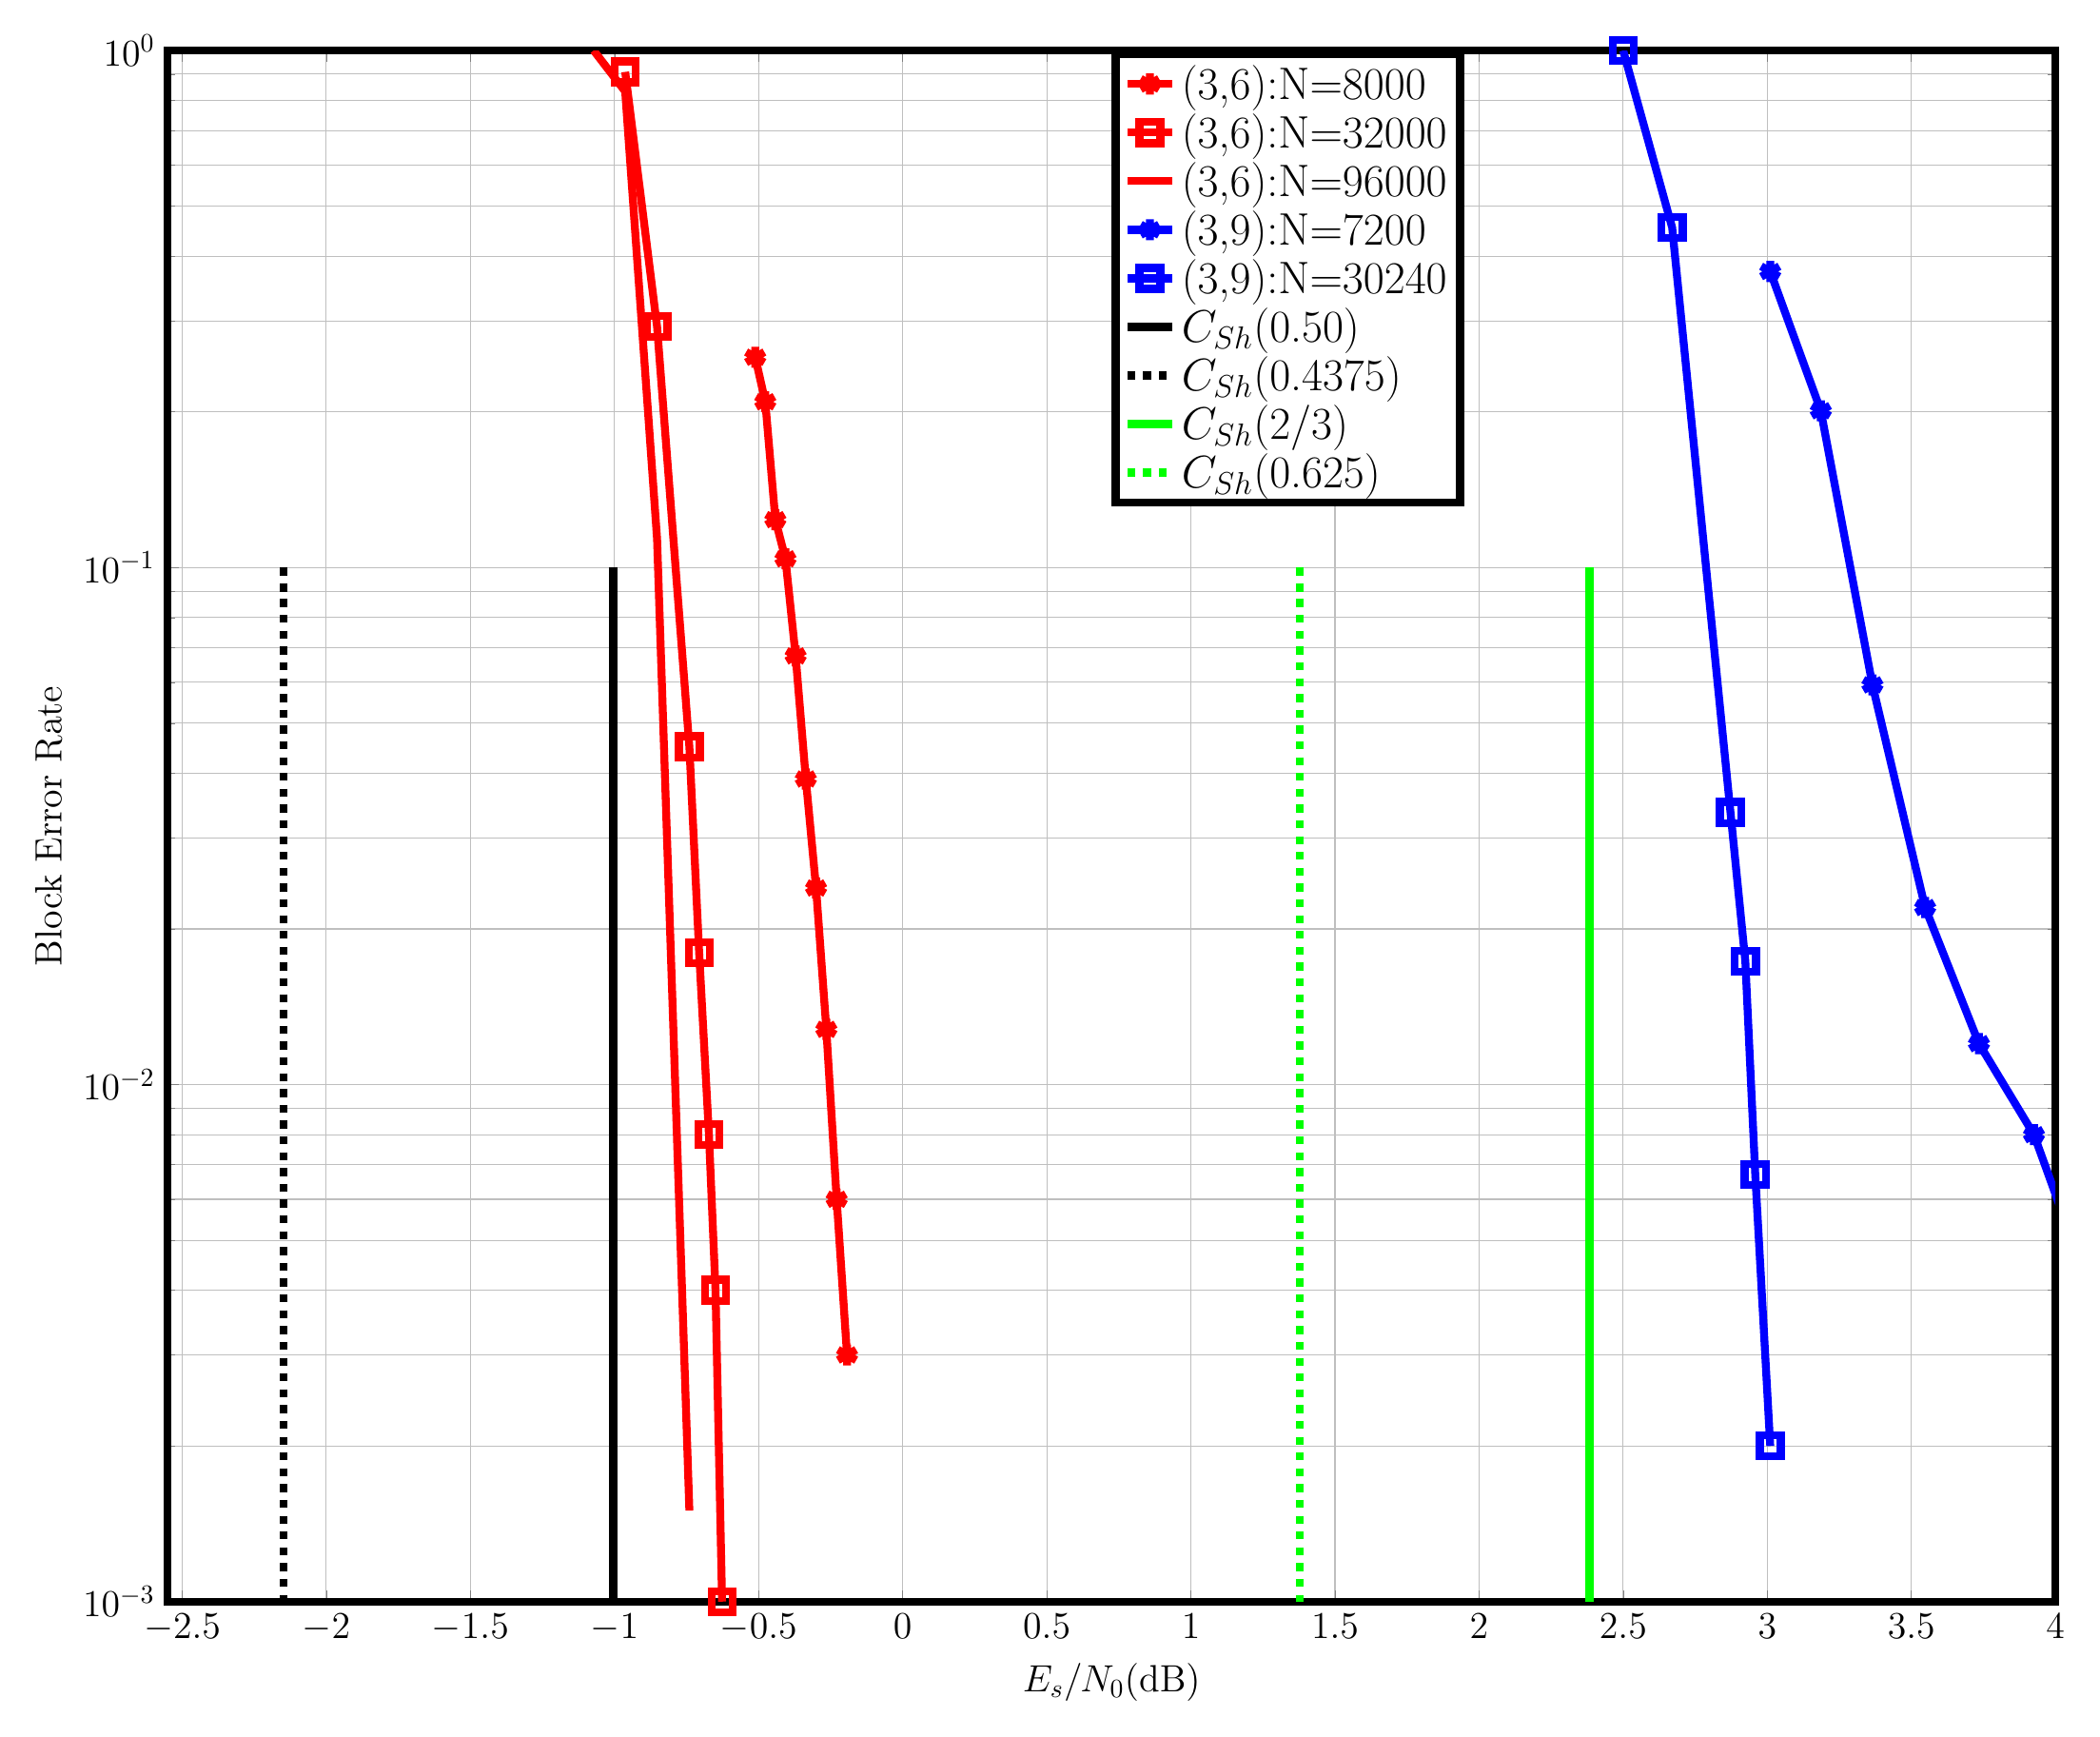
\begin{tikzpicture}
% The SC paramaters for the below set of plots are
% L=16
% w=3.
% So the true rate R is related to design rate R'(=1-dc/dv) as
% 1-R=(L+w-1)*(1-R')/L
\def\fsize{\Large}
\pgfplotsset{every y tick label/.append style={font=\Large}}
\pgfplotsset{every x tick label/.append style={font=\fsize}}

\begin{axis}[%
width=9.91942366579178in,
height=8.14846697287839in,
scale only axis,
xmin=-2.55,
xmax=4,
xtick = {-2.5,-2.0,...,4.5},
xlabel={\fsize{$E_s/N_0$(dB)}},
ylabel={\fsize{Block Error Rate}},
xmajorgrids,
ymode=log,
ymin=0.001,
ymax=1,
yminorticks=true,
ymajorgrids,
yminorgrids,
line width=3.0pt,
legend style={at={(0.5,1)},anchor=north west, draw=black,fill=white,legend cell align=left,font=\LARGE}
]

\addplot [color=red,solid,mark=asterisk,mark size=4.0]
  table[row sep=crcr]{-0.511525224473813	0.255102040816327\\
-0.476711992947787	0.209205020920502\\
-0.441758667557386	0.123762376237624\\
-0.406664116226376	0.103950103950104\\
-0.371427193100643	0.0674763832658569\\
-0.33604673832371	0.039\\
-0.300521577807649	0.024\\
-0.264850522999304	0.0127877237851662\\
-0.229032370641686	0.006\\
-0.193065902530428	0.003\\
};
\addlegendentry{(3,6):N=8000};


\addplot [color=red,solid,mark=square,mark size=4.0]%,mark options={solid}]
  table[row sep=crcr]{
   -0.9628    0.9091\\
   -0.8522    0.2924\\
   -0.7401    0.0450\\
   -0.7062    0.0180\\
   -0.6722    0.0080\\
   -0.6494    0.0040\\
   -0.6266    0.0010\\
 };
\addlegendentry{(3,6):N=32000};

\addplot [color=red,solid,mark=<,mark size=4.0]%,mark options={solid}]
  table[row sep=crcr]{
   -1.0721    1.0000\\
   -0.9628    0.8333\\
   -0.8522    0.1136\\
   -0.7401    0.0015\\
 };
\addlegendentry{(3,6):N=96000};


\addplot [color=blue,solid,mark=asterisk,mark size=4.0]
  table[row sep=crcr]{
   3.0103    0.3738\\
    3.1858    0.2010\\
    3.3649    0.0593\\
    3.5477    0.0220\\
    3.7345    0.0120\\
    3.9254    0.0080\\
    4.1206    0.0040\\
    4.3203    0.0020\\
};
\addlegendentry{(3,9):N=7200};

\addplot [color=blue,solid,mark=square,mark size=4.0]
  table[row sep=crcr]{
	2.50    1.0\\
	2.67   0.4545\\
    2.8724    0.0336\\
    2.9239    0.0173\\
    2.9583    0.0067\\
    3.0103    0.0020\\
};
\addlegendentry{(3,9):N=30240};



\addplot [color=black,solid]
  table[row sep=crcr]{
   -1.0041    0.1000\\
   -1.0041    0.0950\\
   -1.0041    0.0900\\
   -1.0041    0.0850\\
   -1.0041    0.0800\\
   -1.0041    0.0750\\
   -1.0041    0.0700\\
   -1.0041    0.0650\\
   -1.0041    0.0600\\
   -1.0041    0.0550\\
   -1.0041    0.0500\\
   -1.0041    0.0450\\
   -1.0041    0.0400\\
   -1.0041    0.0350\\
   -1.0041    0.0300\\
   -1.0041    0.0250\\
   -1.0041    0.0200\\
   -1.0041    0.0150\\
   -1.0041    0.0100\\
   -1.0041    0.0050\\
   -1.0041    0.0010\\
};
\addlegendentry{$C_{Sh}$(0.50)};

\addplot [color=black,dashed]
  table[row sep=crcr]{
   -2.1477    0.1000\\
   -2.1477    0.0950\\
   -2.1477    0.0900\\
   -2.1477    0.0850\\
   -2.1477    0.0800\\
   -2.1477    0.0750\\
   -2.1477    0.0700\\
   -2.1477    0.0650\\
   -2.1477    0.0600\\
   -2.1477    0.0550\\
   -2.1477    0.0500\\
   -2.1477    0.0450\\
   -2.1477    0.0400\\
   -2.1477    0.0350\\
   -2.1477    0.0300\\
   -2.1477    0.0250\\
   -2.1477    0.0200\\
   -2.1477    0.0150\\
   -2.1477    0.0100\\
   -2.1477    0.0050\\
   -2.1477    0.0010\\
   };
\addlegendentry{$C_{Sh}$(0.4375)};
   
   
   
   
\addplot [color=green,solid]
  table[row sep=crcr]{
    2.3835    0.1000\\
    2.3835    0.0950\\
    2.3835    0.0900\\
    2.3835    0.0850\\
    2.3835    0.0800\\
    2.3835    0.0750\\
    2.3835    0.0700\\
    2.3835    0.0650\\
    2.3835    0.0600\\
    2.3835    0.0550\\
    2.3835    0.0500\\
    2.3835    0.0450\\
    2.3835    0.0400\\
    2.3835    0.0350\\
    2.3835    0.0300\\
    2.3835    0.0250\\
    2.3835    0.0200\\
    2.3835    0.0150\\
    2.3835    0.0100\\
    2.3835    0.0050\\
    2.3835    0.0010\\
    };
\addlegendentry{$C_{Sh}$(2/3)};



\addplot [color=green,dashed]
  table[row sep=crcr]{
	1.3786    0.1000\\
    1.3786    0.0950\\
    1.3786    0.0900\\
    1.3786    0.0850\\
    1.3786    0.0800\\
    1.3786    0.0750\\
    1.3786    0.0700\\
    1.3786    0.0650\\
    1.3786    0.0600\\
    1.3786    0.0550\\
    1.3786    0.0500\\
    1.3786    0.0450\\
    1.3786    0.0400\\
    1.3786    0.0350\\
    1.3786    0.0300\\
    1.3786    0.0250\\
    1.3786    0.0200\\
    1.3786    0.0150\\
    1.3786    0.0100\\
    1.3786    0.0050\\
    1.3786    0.0010\\
        };
\addlegendentry{$C_{Sh}$(0.625)};


   
   
\end{axis}
\end{tikzpicture}%}
  \caption{We simulate the performance of the channel coding component alone using regular $(3,6)$ and $(3,9)$ spatially-coupled LDPC (SC-LDPC) ensembles for increasing block lengths for two user Gaussian MAC channel. The results demonstrate that it is possible to achieve the capacity of two-user GMAC (and can be generalized for $T$-GMAC) using identical code books at all the users.}
  \label{fig:scldpc}
\end{figure}

\subsection{Successive interference cancellation}
\label{sec:SICanalysis}
In the channel coding literature for LDPC codes on binary erasure channel and sparse signals via Tanner graphs literature the symmetric interference cancellation is traditionally studied under the name of peeling decoder which is an iterative process in which if a right node (slot in our case) is connected to only one left node (user) the corresponding left node and all its connections are peeled off from the bipartite graph. This is essentially the symmetric interference cancellation process described in Sec. \ref{Sec:SystemModel} except that we peel off the connections from a right node if the number of variable nodes connected is less than or equal to $T$ instead of $1$. Although density evolution methods are well studied to predict the performance of such decoding processes all the existing density evolution methods are for values of $T=1$. Before we address this issue let us define the considered peeling process precisely.
\begin{definition}[$T$-peeling]
\label{def:T-peeling_process}
We define an ideal SIC decoder as the decoder in which at each slot, if the number of users transmitted and are still undecoded is less than or equal to $T$, then the remaining undecoded users in that slot are decoded with zero error. In other words in the ideal SIC process there are no hash collisions in any slot and the channel and sparse signal decoders are assumed to be zero-error. This process proceeds iteratively until all the users are decoded or there are no slots with undecoded users less than or equal to $T$. We also refer to this as $T$-peeling process.
\end{definition}

\begin{lemma}[Density Evolution (DE)]
Let the left and right degree distributions (d.d.) of the bipartite graph from the edge perspective be $\lambda(x)$ and $\rho(x)$. Then let $x_{t}$ be the probability that an edge in the graph, in iteration $t$ of the $T$-peeling process, is connected to a left node that is undecoded yet. Then the recurrence relation for $x_t$ corresponding to the $T$-peeling process is given by
\begin{align}
y_{t}&=\left[\sum_{r=1}^{T} \rho_r +\sum_{r>T} \rho_r\left( \sum_{t=0}^{T-1}\binom{r-1}{t}(1-x_t)^{r-1-t} x_t^{t}\right) \right],\label{eqn:DE_Tpeeling_check}\\
x_{t+1}&=\lambda(1-y_t).\label{eqn:DE_Tpeeling_bit}
\end{align}
\label{lem:DE_Tpeeling}
\end{lemma}
\begin{proof}
In the context of low density parity check(LDPC) codes the bipartite graph corresponds to the parity check matrix where the left and right nodes represent the bits of the codeword and the parity check equations respectively. If we consider an LDPC code under binary erasure channel where each bit is erased with probability $\epsilon$, under the assumption that the bipartite graph is a tree, the probability that a random edge in the graph is an erasure in iteration $t$ of the peeling process is given by \cite{richardson2008modern}
\begin{align}
y_{t}&=\sum_{r=1}^{r_{\max}} \rho_r (1-x_t)^{r-1}, \label{eqn:DE_LDPC_check}\\
x_{t+1}&=\epsilon \lambda(1-y_t).\label{eqn:DE_LDPC_bit}
\end{align}
Eqn. \eqref{eqn:DE_LDPC_check} is due to the observation that all the incoming messages at a check node are independent, due to the tree assumption, and the outgoing message on an edge from a check node of degree $r$ is a non-erasure if and only if all the incoming messages are non-erasures. For degree distributions with finite maximum degree on the left and right it is shown that a graph chosen randomly from the ensemble $(N,\lambda,\rho)$ is a tree with probability approaching $1$ asymptotically in blocklength of the code.

Now if we consider an edge $e$ connected to check node of degree $r$ in the $T$-peeling process, the outgoing message is a non-erasure if and only if there are at most $T-1$ erasures in the remaining $r-1$ incoming edges. Thus the probability that the outgoing message from a check node of degree $r$ is non-erasure, denoted by $y_{t,r}$, if the incoming message on the remaining $r-1$ edges is an erasure with probability $x_t$ is equal to
%$1-\binom{r-1}{t}(1-x_t)^{r-1-t} x_t^{t}$ if $r>T$ else it is equal to $0$.
\begin{align*}
y_{t,r}&=\sum_{t=0}^{T-1}\binom{r-1}{t}(1-x_t)^{r-1-t} x_t^{t}  ~&\text{if } r>T\\
&=1 ~&\text{else if } r\leq T.
\end{align*}
Averaging over all edges where an edge is connected to a check node of degree $r$ with probability $\rho_r$ gives us Eqn. \eqref{eqn:DE_Tpeeling_check}.
\end{proof}

Let $L(x)=\sum_{i=1}^{l_{\max}} L_i x^i$ be the left d.d according to which the the users choose their repetition parameters as described in Sec. \ref{sec:Txpolicy_TannerGraph} i.e., $\Pr(L_{w}=i)=L_i$. Also let the average left degree of this distribution be $l_{\text{avg}}=\sum_i iL_i$. Then according to our transmission policy the right d.d. $R(x)$ is Binomial distributed with parameters $(\Ka l_{\text{avg}},1/V)$  and in the limit $\Ka\rightarrow \infty$ $R(x)$ can be approximated as Poisson distribution with parameter $r_{\text{avg}}=\frac{\Ka l_{\text{avg}}}{V}$. Thus, asymptotically in $\Ka$, it can be seen that $R(x)=e^{-r_{\text{avg}}(1-x)}$ and $\rho(x)=R'(x)/R'(1)=e^{-r_{\text{avg}}(1-x)}$. For more details refer to \cite{narayanan2012iterative}.

%Let the left d.d from node  and edge perspective be $L(x)$ and $\lambda(x)$ respectively.
\begin{lemma} For $V=\alpha K_a$ where $\alpha$ is fixed the asymptotic performance of our transmission scheme under the ideal SIC decoding process can be characterized by %and in the limit $\Ka\rightarrow\infty$, the SIC process recovers atleast $(1-\epsilon_0)$ fraction of the users with high probability for values of
\begin{align*}
\lim_{\Ka\rightarrow \infty} \Pr(\mc{E}_{\text{SIC}}(\Ka,T))&=L(1-y_{\infty})\notag\\
\text{ where } y_{\infty} &=\lim_{t\rightarrow\infty} y_t,
\end{align*}
and $\Pr(\mc{E}_{\text{SIC}}(\Ka,T))$ is the probability that the ideal SIC process does not recover a user given there  are $K_a$ users. Here the initial condition is $x_0=1$ and the evolution of $x_t,y_t$ is given by the DE relationship in Lem. \ref{lem:DE_Tpeeling}.
\label{lem:asymptotic_SIC}
\end{lemma}

\begin{figure}[h!]
  \centering
  \resizebox{0.85\textwidth}{!}{% This file was created by matlab2tikz v0.4.7 running on MATLAB 7.14.
% Copyright (c) 2008--2014, Nico Schlömer <nico.schloemer@gmail.com>
% All rights reserved.
% Minimal pgfplots version: 1.3
% 
% The latest updates can be retrieved from
%   http://www.mathworks.com/matlabcentral/fileexchange/22022-matlab2tikz
% where you can also make suggestions and rate matlab2tikz.
% 
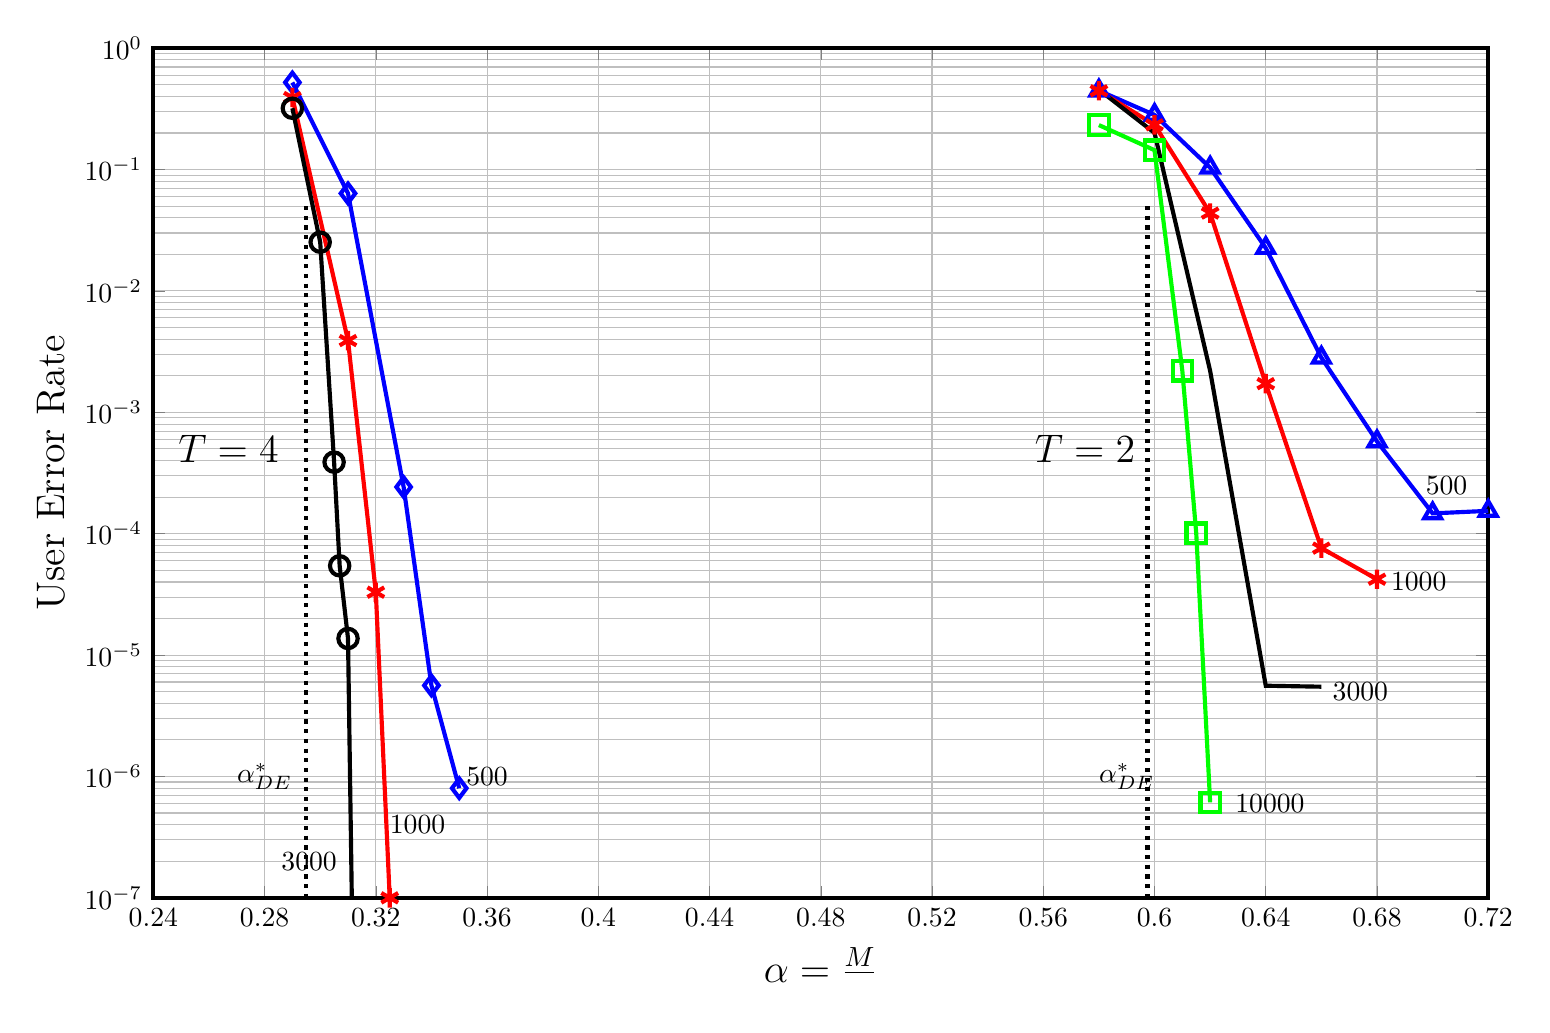
\begin{tikzpicture}
\def\fsize{\Large}

\begin{axis}[%
width=7.2971708223972in,
height=4.87099759405074in,
xmin=0.24,
xmax=0.72,
xmajorgrids,
xtick={0.16,0.20,...,0.8},
xlabel={\fsize $\alpha=\frac{M•}{\Ka}$},
ymode=log,
ymin=1e-07,
ymax=1,
yminorticks=false,
ymajorgrids,
ylabel={\fsize User Error Rate},
yminorgrids,
line width=1.5pt,
mark size=3.5pt,
legend style={at={(0.4,1)},anchor=north, draw=black,fill=white,legend cell align=left,font=\normalsize}
]

\node[] at (axis cs: 0.267,5e-4) {\fsize $T=4$};
\node[] at (axis cs: 0.28,1e-6) {$\alpha^*_{\text{DE}}$};
\node[] at (axis cs: 0.36,1e-6) {$500$};
\node[] at (axis cs: 0.335,4e-7) {$1000$};
\node[right] at (axis cs: 0.282,2e-7) {$3000$};


\node[] at (axis cs: 0.59,1e-6) {$\alpha^*_{\text{DE}}$};
\node[] at (axis cs: 0.575,5e-4) {\fsize $T=2$};
\node[] at (axis cs: 0.705,2.5e-4) {$500$};
\node[] at (axis cs: 0.695,4e-5) {$1000$};
\node[right] at (axis cs: 0.66,5e-6) {$3000$};
\node[right] at (axis cs: 0.625,6e-7) {$10000$};

\addplot [color=blue,solid,mark=triangle]
  table[row sep=crcr]{
0.58	0.446855769230769\\
0.6	0.281691729323308\\
0.62	0.103645655877342\\
0.64	0.0225469613259669\\
0.66	0.00281948757763975\\
0.68	0.00057567726737338\\
0.7	0.000146973130462933\\
0.72	0.00015425828775533\\
%0.74	0.000138459944035651\\
};
%\addlegendentry{$(T,\lambda,\Ka)=(2,0,500)$};
%\addlegendentry{$\Ka=500$};

\addplot [color=red,solid,mark=asterisk,mark options=solid]
  table[row sep=crcr]{
0.58	0.445524509803922\\
0.6	0.233573333333333\\
0.62	0.0437690582959641\\
0.64	0.00172267248545303\\
0.66	7.60343481654957e-05\\
0.68	4.21380449980933e-05\\
%0.7	3.98492524403806e-05\\
%0.72	3.09173107773079e-05\\
%0.74	2.93069123570536e-05\\
};
%\addlegendentry{$(T,\lambda,\Ka)=(2,0,1000)$};
%\addlegendentry{$\Ka=10^3$};

\addplot [color=black,solid,mark=circle,mark options=solid]
  table[row sep=crcr]{
0.58	0.45552736318408\\
0.6	0.200620588235294\\
0.62	0.00219567231339333\\
0.64	5.59111903411393e-06\\
0.66	5.48796389541606e-06\\
%0.68	4.02e-06\\
};
%\addlegendentry{$(T,\lambda,\Ka)=(2,0,3000)$};\\
%\addlegendentry{$\Ka=3\times 10^3)$};

\addplot [color=green,solid,mark=square,mark options=solid]
  table[row sep=crcr]{
0.58	    0.2324    \\
0.60     0.1444\\
0.61	    0.0022\\
0.615	1.009e-4\\
0.62		6.12e-7\\
};
%\addlegendentry{$(T,\lambda,\Ka)=(2,0,10000)$};
%\addlegendentry{$\Ka=10^4$};


\addplot [color=black,dotted]
  table[row sep=crcr]{
0.5975	5.00e-2 \\
0.5975	1.00e-2 \\
0.5975	5.00e-3 \\
0.5975	1.00e-3 \\
0.5975	5.00e-4 \\
0.5975	1.00e-4 \\
0.5975	5.00e-5 \\
0.5975	1.00e-5 \\
0.5975	5.00e-6 \\
0.5975	1.00e-6 \\
0.5975	1.00e-7 \\
};
%\addlegendentry{$\alpha_{\text{DE}}$ for $(T,\lambda)=(2,0)$};



%%%%%%%%%-----------------------%----------------------------------
\addplot [color=blue,solid,mark=diamond]
  table[row sep=crcr]{
0.29   0.522000000000000\\
0.31  0.063631578947368\\
0.33  0.000242494494030\\
0.34  5.6200e-6\\
0.35  0.000000800000000\\
   };
%\addlegendentry{$(T,\lambda,\Ka)=(4,0,500)$};
%\addlegendentry{$\Ka=500$};

\addplot [color=red,solid,mark=asterisk,mark options=solid]
  table[row sep=crcr]{
0.2900    0.3920\\
0.3100    0.0039\\
0.3200    3.295189e-5\\
0.3250    1.000e-7\\
    };
%\addlegendentry{$(T,\lambda,\Ka)=(4,0,1000)$};
%\addlegendentry{$\Ka=10^3$};

\addplot [color=black,solid,mark=o,mark options=solid]
  table[row sep=crcr]{
0.2900    0.3198\\
0.30        2.5202e-2\\
0.305      3.88695e-4\\
0.307      5.4376e-5\\
%0.309      2.70211e-5\\
0.310     1.370211e-5\\
0.312     1.02e-8\\
    };
%\addlegendentry{$(T,\lambda,\Ka)=(4,0,3000)$};
%\addlegendentry{$\Ka=3\times 10^3$};


\addplot [color=black,dotted]
  table[row sep=crcr]{
0.2949	5.00e-2 \\
0.2949	1.00e-2 \\
0.2949	5.00e-3 \\
0.2949	1.00e-3 \\
0.2949	5.00e-4 \\
0.2949	1.00e-4 \\
0.2949	5.00e-5 \\
0.2949	1.00e-5 \\
0.2949	5.00e-6 \\
0.2949	1.00e-6 \\
0.2949	5.00e-7 \\
0.2949	1.00e-7 \\
};
%\addlegendentry{$\alpha_{\text{DE}}$ for $(T,\lambda)=(4,0)$};

\end{axis}
\end{tikzpicture}}
  \caption{$\alpha^*_{\text{DE}}$ is the density evolution threshold computed for $L(x)=x^2$ and $T=\{2,4\}$ from Lemmma. \eqref{lem:DE_Tpeeling}. We validate the threshold behavior by evaluating the $T$-peeling performance via Monte Carlo simulations for increasing blocklengths. We observe that the simulations indeed confirm the threshold behavior for values of $\alpha$ above the DE threshold.}
  \label{fig:DEvBP}
\end{figure}

As we can see from Eqns. \eqref{eqn:DE_Tpeeling_bit} and \eqref{eqn:DE_Tpeeling_check} that $x_t=0$ is a fixed point if and only if $\lambda_0=0$. This leads us to the following result characterizing he threshold behavior of the system.
\begin{definition}[Density Evolution Threshold]
If $L_1=0$ we define the density evolution threshold $\alpha^*_{\text{DE}}$ to be
\[
\alpha^*_{\text{DE}}\defeq \inf \{\alpha: \lim_{\Ka\rightarrow \infty} \Pr(\mc{E}_{\text{SIC}}(\Ka,T))=0\}.
\]
\label{def:DE_threshold}
\end{definition}

We validate the threshold behavior via simulations.  For a fixed left d.d $L(x)=x^2$ we first compute the density evolution thresholds according to Def.~\ref{def:DE_threshold} to be $0.5975$ and $0.2949$ for $T=2,4$ respectively. We then perform Monte Carlo simulations where each time a random graph is chosen as described in Sec. \ref{sec:Txpolicy_TannerGraph} for increasing values of $\Ka$ and plot the performance as we incrase the number of slots. The results are presented in Fig.~\ref{fig:DEvBP}. In both the cases the threshold behavior can be clearly seen that as $\Ka$ increases the probability of a user not being decoded decreases sharply for values of $\alpha>\alpha_{\text{DE}}^*$ and remains fairly constant for values of $\alpha\leq\alpha_{\text{DE}}^*$.

\section{Numerical results}
In this section we numerically evaluate the overall performance of the proposed scheme and compare with other multiple access schemes available in the literature. In \cite{ordentlich2017low} apart from proposing a low complexity coding scheme for the unsourced GMAC channel the authors Ordentlich and Polyanskiy also evaluate the performance of their proposed scheme by computing the minimum SNR required to achieve the target error probability for a fixed set of parameters. To make the comparison convenient we pick identical parameters, summarized as following:
\begin{itemize}
\item number of bits each user intends to transmit $B=100$
\item total number of channel uses $\tilde{N}=30,000$
\item number of active users $\Ka\in [25:300]$
\item maximum per user error probability $P_e\leq \epsilon=0.05$.
\end{itemize}

With the parameters $B,\tilde{N},\Ka,\epsilon$ fixed, the choices for the design parameters are as following:
\begin{enumerate}
\item Maximum number of users to be jointly decoded at a slot $T\in\{2,4,5\}$.
\item  The left d.d is chosen to be $L(x)=\beta x+(1-\beta)x^2$ (see Remark~\ref{rmrk:mindegreeisone}). The free parameter is optimized over the set $\beta\in\{0,0.1,\ldots,1\}$. 
\item Number of preamble and channel coding message bits: $\Bp=9,~\Bc=B-\Bp=91$. 
\item \textit{Sensing matrix for preamble component}: Note that $\Mp=2^{\Bp}=512$ is the size of the sensing matrix $\mathbf{A}$. We choose the sensing matrix of dimensions $\Np \times \Mp=63\times 512$ as described in Ex.~\ref{ex:sensingmatrix_BCHsubset}.
% Let binary code $\mc{C}_{\text{BCH}}$ be the BCH$(63,10)$ code of size $1024$. We obtain a subset of $\mc{C}_{\text{BCH}}$ of size $M_\mathrm{p}$ by the following decomposition
%\[
%\mc{C}_{\text{BCH}}=\mc{C}_0\cup \mc{C}_1 ~~\text{ such that } c\in \mc{C}_1 \iff \bar{c}\in\mc{C}_0,
%\]
%where $\bar{c}=\mathbf{1}\oplus c$ i.e., the one's complement of $c$. We choose the sensing matrix of size $\Np \times \Mp=63\times 512$ as
%\begin{align}
%\mathbf{A}=[\av_1,\av_2,\ldots,\av_{M_\mathrm{p}}],
%\label{eqn:sensingMatrix_defn}
%\end{align}
%where $\av_i=\sqrt{\Pp}(1-2\cv_i), \cv_i\in\mc{C}_1$, i.e., $a_{ij}\in\{-\sqrt{\Pp},\sqrt{\Pp}\} \forall i,j$.
%Let $\mc{C}_0$ be the binary code of size $2^9$ described in Ex.~\ref{Ex:BCH_halfcode}.
\item \textit{Channel coding component}: The number of channel uses available for channel coding $\Nc$ is dependent on $N$ which in turn depends on the total number of sub-blocks $V$. It is impractical to build a channel code for various rates $R_{\mathrm{c}}=\frac{\Bc}{\Nc}$ (although $\Bc$ is fixed, $\Nc$ needs to be optimized over) and evaluate the performance numerically for each set of parameters ($\Nc,\Bc$). Therefore to evaluate the performance of the channel coding component we use the finite block length achievability bound in Eqn. \eqref{Eqn:Polyanskiy_miniresult} due to Polyanskiy. This seems a reasonable choice as we demonstrated in Fig. xx that one can construct LDPC codes even for moderate block lengths that perform close to the above mentioned bound.
\end{enumerate}

%\item
 From Eqn. \ref{eqn:errPrb_split} we want $\Pr(\mc{E}'_{\text{SIC}})+V\left(\Pr(\mc{E}_{\mathrm{p}})+\Pr(\mc{E}_{\mathrm{e}})+\Pr(\mc{E}_{\mathrm{c}})\right)\leq \epsilon=0.05$. Therefore we set the target error probabilities for the individual events as $\Pr(\mc{E}_i)\leq \epsilon_0/3/V$, $i\in\{\mathrm{p},\mathrm{e},\mathrm{c}\}$ where we choose $\epsilon_0=0.01$ and $\Pr(\mc{E}'_{\text{SIC}})\leq (\epsilon-\epsilon_0)=0.04$. For a fixed $T$ the performance of the overall scheme i.e., the minimum $E_b/N_0$ required for achieving $P_e\leq\epsilon$ is computed as following:
\begin{align}
\frac{E_b}{N_0}=\min_{\beta} \frac{(2-\beta)(\Np \Pp+\Nc\Pc)}{2B}
\label{eqn:EbN0_computation}
\end{align}
where
\begin{align}
\Pp&\coleq \arg\min_{P}~ \max \left(\Pr(\mc{E}_{\mathrm{p}}),\Pr(\mc{E}_{\mathrm{e}}) \right)\leq \frac{\epsilon_0}{3V}\label{eqn:PrE3_sims}\\
\Pc&\coleq \arg\min_{P}~\hFBL(N,B_\mathrm{c},T,P))\leq \frac{\epsilon_0}{3V}\qquad (\text{see Eqn. }\eqref{eqn:FBLbounds})  \label{eqn:PrFBL_sims}\\
N&\coleq\left\lfloor \frac{\tilde{N}}{V}\right\rfloor \notag\\
V&\coleq \arg\min_{V}~\Pr(\mc{E}'_{\text{SIC}}(\Ka,V,T))\leq \epsilon-\epsilon_0\label{eqn:PrESIC_sims}.
\end{align}
A remark on how we compute the quantities in Eqns. \eqref{eqn:PrE3_sims}, \eqref{eqn:PrFBL_sims} and \eqref{eqn:PrESIC_sims}:
\begin{itemize}
\item $\Pr(\mc{E}_{\mathrm{p}}):$ We choose $T$ preamble message indices, randomly, without replacement from the available $M_\mathrm{p}$ indices and form the measurement vector. We then use the list decoder as described in Sec. \ref{sec:CS_decoder}. The probability of error $\Pr(\mc{E}_{\mathrm{p}})$ in Eqn. \eqref{eqn:PrE3_sims} is then computed from atleast $10^5$ Monte Carlo simulations
\item $\Pr(\mc{E}_{\mathrm{c}})$: We use the upper bound for $\Pr(\mc{E}_{\mathrm{c}})$ given in Lem.~\ref{lem:energytest_overallerror} except for the term 
\[
\Pr\left( \frac{1}{\Np}||\av_i+\av_j+\zv||^2\leq (1+\Pp)\right)
\]
which we evaluate numerically from atleast $10^5$ Monte Carlo simulations. In each simulation we choose indices $i,j$ randomly without replacement from the set $[\Mp]$ and $\zv\sim \mc{N}(0,\mathbf{I}_{\Np})$.
\item $\Pr(\mc{E}'_{\text{SIC}}(\Ka,V,T))$: We rely on Monte Carlo simulations wherein for each simulation we generate a bipartite graph of $\Ka$ variable nodes and $V$ slot nodes with edge connections as described in Sec. \ref{sec:Txpolicy_TannerGraph}. We run the simplified SIC decoder on just the bipartite graph as described in Def.~\ref{def:simple_SIC} and evaluate the per user error probability. 
\end{itemize}
Finally the results for the minimum SNR required to achieve the target error probability optimized according to Eqn. \eqref{eqn:EbN0_computation} are presented in Fig. \ref{fig:simulationresults_new}.
 
\begin{figure}[!ht]
\centering
 \resizebox{0.85\textwidth}{!}{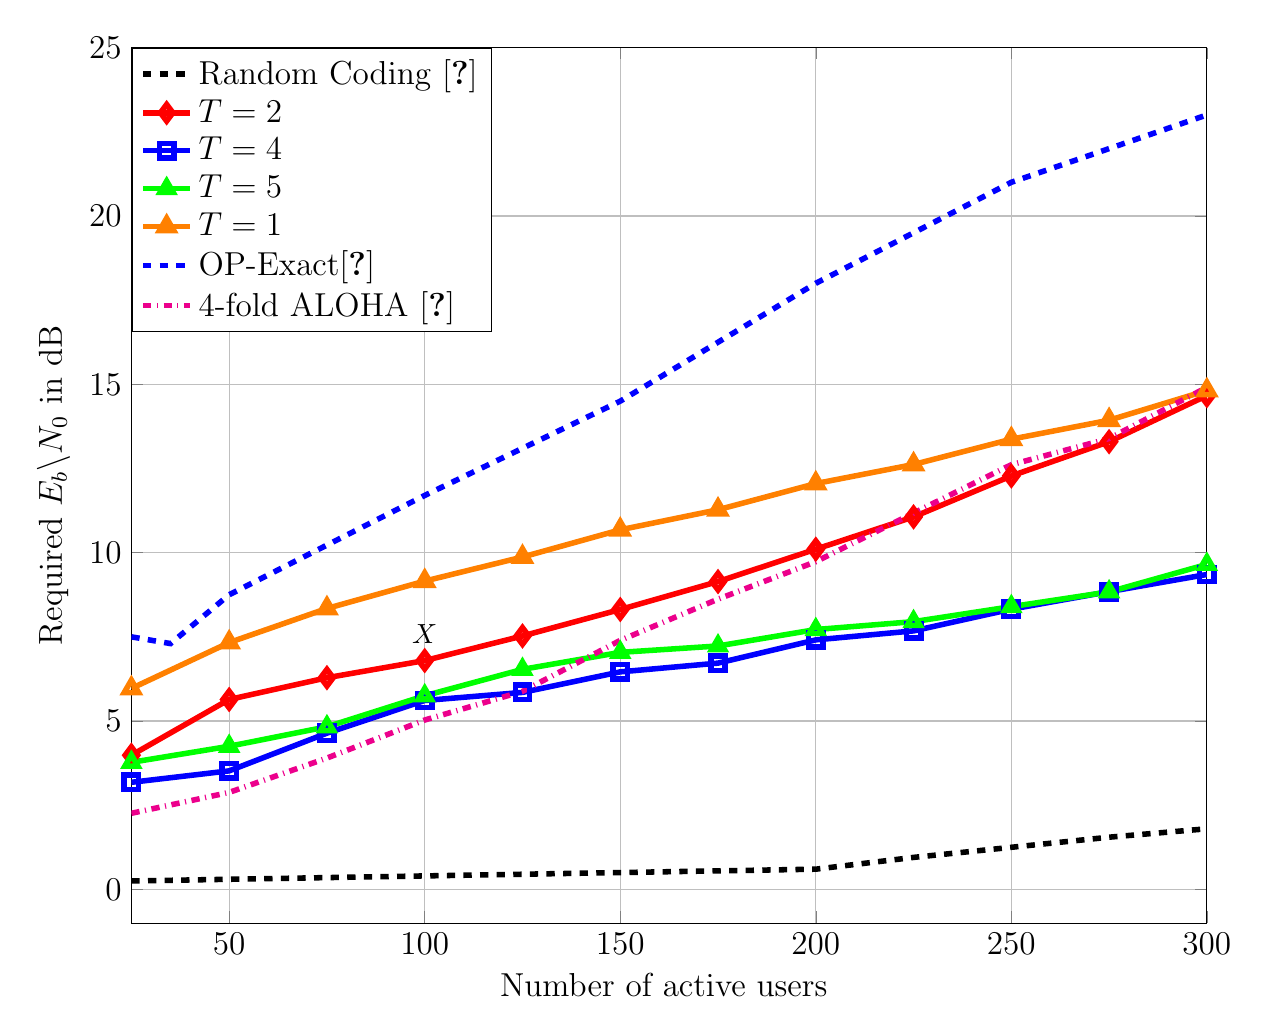
\begin{tikzpicture}
\def\fsize{\large}
\pgfplotsset{every y tick label/.append style={font=\fsize}}
\pgfplotsset{every x tick label/.append style={font=\fsize}}

\begin{axis}[%
width=6in,
height=5in,
xmin=25,
xmax=300,
xtick = {50,100,...,300},
xlabel={\fsize{Number of active users $\Ka$}},
ylabel={\fsize{Required $E_b\backslash N_0$ in dB}},
xmajorgrids,
xminorgrids,
ymin=-1,
ymax=25,
ytick = {-5,0,...,30},
yminorticks=true,
ymajorgrids,
yminorgrids,
legend style={at={(0,1)},anchor=north west, draw=black,fill=white,legend cell align=left,font=\fsize}
]

\node[] at (axis cs: 100,7.5696) {$X$};

\addplot [color=black,solid,dashed, line width=2.0pt]
  table[row sep=crcr]{
  25     0.25\\
 50     0.3\\
 75     0.35\\
100     0.4\\
125     0.45\\
150     0.5\\
175    0.55\\
200  0.60\\
225 0.95\\
250 1.25\\
275 1.55\\
300 1.8\\
};
\addlegendentry{Random Coding \cite{polyanskiy2017perspective} };

\addplot [color=red,solid,mark=diamond,mark size=3.0, line width=2.0pt]
  table[row sep=crcr]{
  25   3.9849  \\
  50   5.6396\\
  75   6.2855  \\
100  6.7952 \\
125  7.5262 \\
150  8.3122 \\
175  9.1418 \\
200  10.103 \\
225  11.062 \\
250  12.279 \\
275 13.296 \\
300 14.6648 \\
};
\addlegendentry{$T=2$};

\addplot [color=blue,solid,mark=square,mark size=2.6, line width=2.0pt]
  table[row sep=crcr]{
 25 3.18\\
 50 3.52\\
 75 4.64\\
100 5.61\\
125 5.85\\
150 6.46\\
175 6.72\\
200 7.41\\
 225 7.6772\\
 250 8.3217\\
 275 8.8428\\
 300 9.3520 \\
};
\addlegendentry{$T=4$};

%\addplot [color=blue,dotted, line width=2.0pt]
%  table[row sep=crcr]{
% 25 2.8815\\
% 50 3.2015\\
% 75 4.3960\\
%100 5.30\\
%125 5.5533\\
%150 6.1838\\
%175 6.4562\\
%200 7.1900\\
% 225 7.4664\\
% 250 8.1394\\
% 275 8.6810\\
% 300 9.2079 \\
%};
%\addlegendentry{$T=4$,ML-CS};

\addplot [color=green,mark=triangle,mark size=2.7, line width=2.0pt]
  table[row sep=crcr]{
 25 3.7732\\
 50 4.25\\
 75 4.8287\\
100 5.7503\\
125 6.5344\\
150 7.0391\\
175 7.2288\\
200 7.7171\\
 225 7.9514 \\
250 8.3968\\
275 8.8358\\
300  9.6524\\
};
\addlegendentry{$T=5$};

\addplot [color=orange,solid,mark=triangle,mark size=3.0, line width=2.0pt]
table[row sep=crcr]{
25 5.9675\\
50 7.33\\
75 8.3433\\
100 9.1555\\
125 9.8708\\
150 10.679\\
175 11.275\\
200 12.052 \\
225 12.61860 \\
250 13.3702 \\
275 13.934\\
300 14.816\\
 };
\addlegendentry{$T=1$}; %After Yury's correction



\addplot [color=blue,dashed, line width=2.0pt]
  table[row sep=crcr]{
  25   7.50 \\
   35   7.30 \\
  50   8.75 \\
  100 11.7 \\
  150 14.50\\
%175  6.7814 \\
200  18\\
%225  7.6838 \\
250  21\\
%275  8.4960 \\
300 23\\
};
\addlegendentry{OP-Exact\cite{ordentlich2017low}};

\addplot [color=magenta,dash dot,line width=2.0pt]
  table[row sep=crcr]{
  25   2.26  \\
  50   2.88  \\
  75   3.90  \\
 100   5.03 \\
  125.0000    5.8798 \\
  150.0000    7.3954 \\
  175.0000    8.6199 \\
  200.0000    9.7328 \\
  225.0000   11.1761\\
  250.0000   12.6127\\
  275.0000   13.3907\\
  300.0000   14.9116\\
  };
\addlegendentry{4-fold ALOHA \cite{ordentlich2017low}};

\end{axis}
\end{tikzpicture}}
  \caption{Minimum $E_b/N_0$ required to achieve $P_e\leq 0.05$ as a function of number of users. The x mark represents the performance of our proposed scheme where for the channel coding part instead of the finite blocklength bounds given in \cite{polyanskiy2017perspective}, we use numerical simulation results from a regular LDPC code.}
  \label{fig:simulationresults_new}
%\end{minipage}
\end{figure}
 
In Fig.~\ref{fig:simulationresults_new} the curves labelled $T=2$, $T=4$ and $T=5$ correspond to the performance of our proposed scheme evaluated as described above for various values of parameter $T$. The curve labelled 4-fold ALOHA is the performance of the 4-fold ALOHA scheme from \cite{ordentlich2017low}.
% wherein  assumes exactly the same code.
 It can be seen that for large values of $\Ka$, our proposed scheme with $T=4$ or $5$ substantially outperforms the 4-fold ALOHA and this gain is due to the iterative decoding process that is absent in 4-fold ALOHA. The curve labelled OP-Exact is a reproduction of the results from \cite{ordentlich2017low} of the practical scheme introduced there. 
 
 The x mark represents our proposed scheme where for the channel coding part instead of the FBL bounds we use the actual simulation results. We use a rate-1/4 $(364,91)$ LDPC code obtained from repeating every coded bit of (3,6) LDPC code twice and a message passing decoder for $T=2$. It can be seen that the simulation results with the $(3,6)$ LDPC code are only 0.5~dB away from the curve corresponding to $T=2$ showing that the pragmatic coding scheme can perform close to the finite length bounds. It can also be seen that our proposed scheme provides substantial gain over the results in \cite{ordentlich2017low}.
 
In the proposed encoding scheme, for $L(x)=\beta x+(1-\beta)x^2$ each user may transmit once or twice depending on the message index chosen. We need to point out that the power constraint employed is an average over all the message indices i.e
\[
\mathbb{E}_{w}\left[||\cv_w||^2\right]=(2-\beta)P.
\]
We also present the results when the power constraint is uniform across all the codewords in the code i.e., $||\cv_w||^2\leq P \forall w$ in Fig.~\ref{fig:simulationresults30000}. We achieve this, for each value of SNR $E_s/N_0$, by choosing $\beta=0$( or $1$) which in turn guarantees each codeword is repeated exactly twice (or once) irrespective of the message.

\begin{remark}
\label{rmrk:mindegreeisone}
Although in Sec. \ref{sec:SICanalysis} we remarked that if the minimum left degree is one then zero is not a fixed point for the DE equations or in other words, in the asymptotic regime, we will have error floors rather than threshold behavior. But the effects of a minimum left degree of one in the finite number of users regime are not very clear. 
\end{remark}


%of our proposed scheme for assuming the existence of a coding scheme for the $T$-user multiple access channel 
%that achieves the finite block length(FBL) bounds in \cite{polyanskiy2017perspective}.
%The authors with ALOHA, treating inference as noise (TIN), and the random coding achievability bounds. The performance of OP-Exact is already substantially better than many other multiple access schemes and our proposed scheme can potentially provide more than 14~dB improvement over OP-Exact for large values of $\Ka$ and is only about 7~dB away from Polyanskiy's FBL bound \cite{polyanskiy2017perspective}. The slope of the $T=4$ curve also is much closer to the finite block length bound which is encouraging for larger values of $K_a$. 

%\subsection*{Further comments:}
%\begin{enumerate}
%\item In bounding the error probability of GMAC decoder in Eqn. \eqref{eqn:PrFBL_sims} we employ the finite blocklength bounds instead of the actual simulations using the LDPC codes as described in encoding section. As we can see from Fig. \ref{fig:BP_simulations} these family of codes at moderate blocklengths $8\times 10^3-10^5$ under the computationally efficient parallel BP decoder have performance very close to the Shannon limit. But as widely known these codes are not the best choice of codes at the blocklengths in consideration for the problem i.e., $\approx 300-1000$.
%\item


\begin{figure}[h]
\centering
 \resizebox{0.75\textwidth}{!}{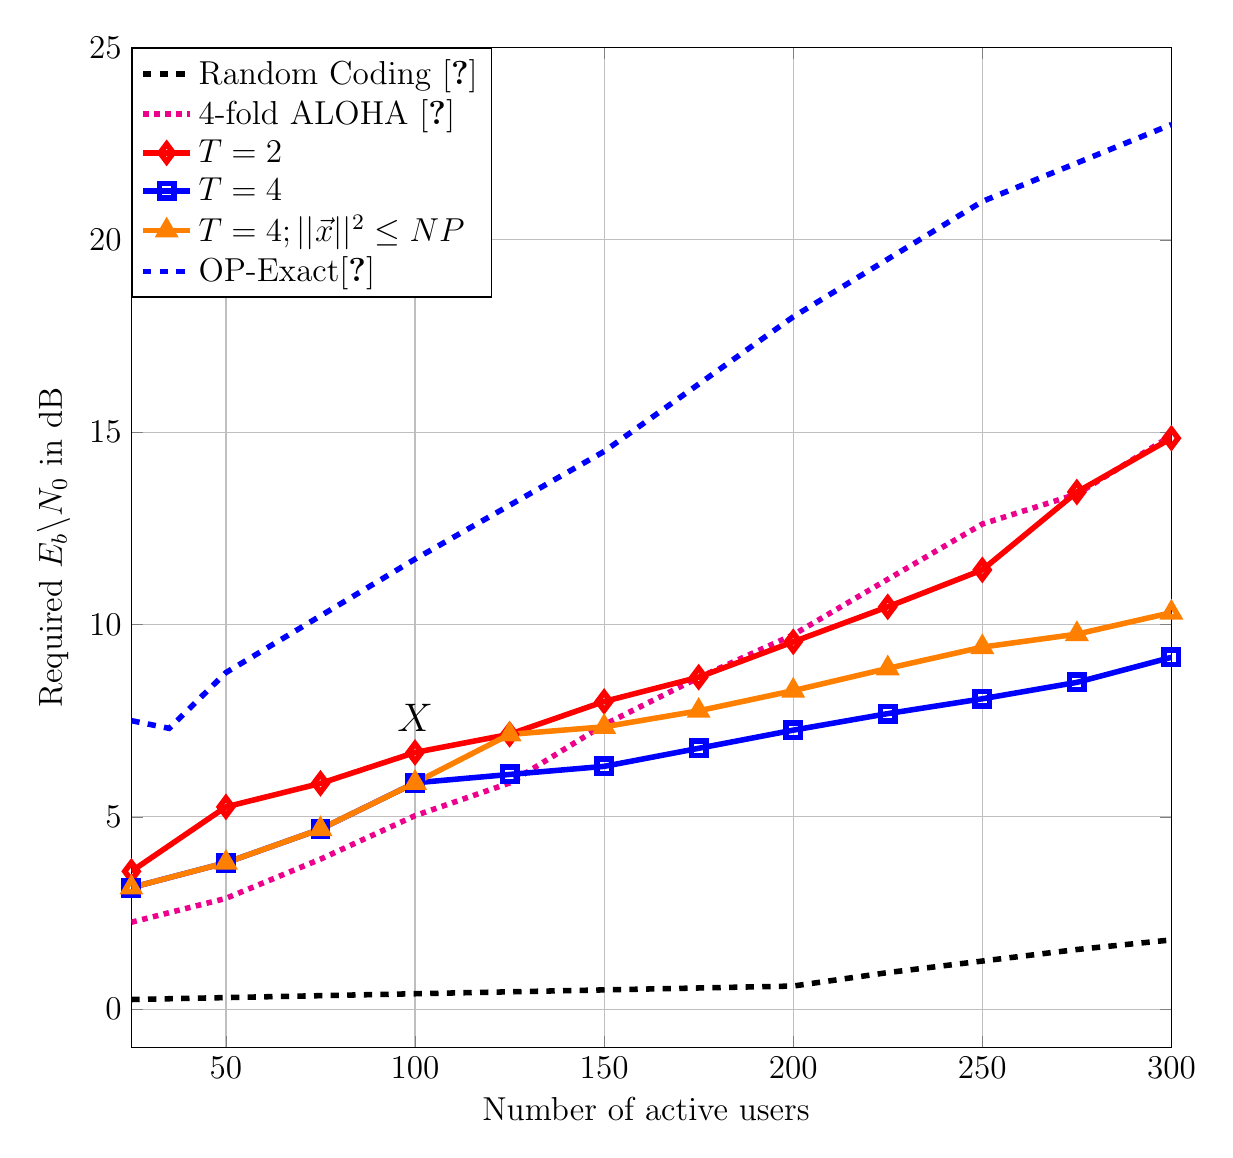
\begin{tikzpicture}
% The SC paramaters for the below set of plots are
% L=16
% w=3.
% So the true rate R is related to design rate R'(=1-dc/dv) as
% 1-R=(L+w-1)*(1-R')/L
\def\fsize{\large}
\pgfplotsset{every y tick label/.append style={font=\fsize}}
\pgfplotsset{every x tick label/.append style={font=\fsize}}

\begin{axis}[%
width=5.2in,
height=5in,
scale only axis,
xmin=25,
xmax=300,
xtick = {50,100,...,300},
xlabel={\fsize{Number of active users $\Ka$}},
ylabel={\fsize{Required $E_b\backslash N_0$ in dB}},
xmajorgrids,
xminorgrids,
ymin=-1,
ymax=25,
ytick = {-5,0,...,30},
yminorticks=true,
ymajorgrids,
yminorgrids,
legend style={at={(0,1)},anchor=north west, draw=black,fill=white,legend cell align=left,font=\fsize}
]

\node[] at (axis cs: 100,7.5696) {\Large $X$};

\addplot [color=black,solid,dashed, line width=2.0pt]
  table[row sep=crcr]{
  25     0.25\\
 50     0.3\\
 75     0.35\\
100     0.4\\
125     0.45\\
150     0.5\\
175    0.55\\
200  0.60\\
225 0.95\\
250 1.25\\
275 1.55\\
300 1.8\\
};
\addlegendentry{Random Coding \cite{polyanskiy2017perspective} };

\addplot [color=magenta,dotted,line width=2.0pt]
  table[row sep=crcr]{
  25   2.26  \\
  50   2.88  \\
  75   3.90  \\
 100   5.03 \\
  125.0000    5.8798 \\
  150.0000    7.3954 \\
  175.0000    8.6199 \\
  200.0000    9.7328 \\
  225.0000   11.1761\\
  250.0000   12.6127\\
  275.0000   13.3907\\
  300.0000   14.9116\\
  };
\addlegendentry{4-fold ALOHA \cite{ordentlich2017low}};

\addplot [color=red,solid,mark=diamond,mark size=3.2,line width=2.0pt]
  table[row sep=crcr]{
  25   3.5820  \\
  50   5.2585 \\
  75   5.8700  \\
100  6.6738 \\
125  7.1463 \\
150  7.9984 \\
175  8.63 \\
200  9.55 \\
225  10.46 \\
250  11.42 \\
275 13.4438 \\
300 14.8439 \\
};
\addlegendentry{$T=2$};

\addplot [color=blue,solid,mark=square,mark size=2.6,line width=2.0pt]
  table[row sep=crcr]{
 25 3.1608  \\
 50 3.8064 \\ %lambda=1.0
 75 4.6803\\
100 5.8835\\
125  6.1017 \\
150  6.3117 \\
175  6.7814 \\
200  7.2532 \\
225  7.6838 \\
250  8.0691\\
275  8.4960 \\
300 9.1467 \\
};
\addlegendentry{$T=4$};

\addplot [color=orange,solid,mark=triangle,mark size=3.0,line width=2.0pt]
  table[row sep=crcr]{
 25 3.1608  \\
 50 3.8064 \\
 75 4.6803\\
100 5.8835\\
125 7.1428\\
150 7.3395\\
175 7.7561\\
200 8.2802 \\
225 8.8590 \\
250 9.4124 \\
275 9.7502\\
300 10.3086\\
 };
\addlegendentry{$T=4;||\vec{x}||^2\leq NP$};



\addplot [color=blue,dashed,line width=2.0pt]
  table[row sep=crcr]{
  25   7.50 \\
   35   7.30 \\
  50   8.75 \\
  100 11.7 \\
  150 14.50\\
%175  6.7814 \\
200  18\\
%225  7.6838 \\
250  21\\
%275  8.4960 \\
300 23\\
};
\addlegendentry{OP-Exact\cite{ordentlich2017low}};

\end{axis}
\end{tikzpicture}


%Old result with error in random_coding_GMAC: used log2 instead of log
%\addplot [color=red,solid,mark=diamond,mark size=4.0]
%  table[row sep=crcr]{
%  25   2.1522  \\
%  50   4.0581\\
%  75   4.5625\\
%100  5.3325 \\
%125    5.4330\\
%150  5.8549 \\
%175  6.3787\\
%200  6.6580 \\
%225  7.9109\\
%250  8.5476\\
%275   9.5476\\
% 300 10.3177\\
%};
%\addlegendentry{T=2};

%\addplot [color=blue,solid,mark=square,mark size=3.0]
%  table[row sep=crcr]{
% 25 2.1178\\
% 50 2.6828\\
% 75 3.1482 \\
%100 3.7733\\
%125 4.6866\\
%150 5.4191\\
%175 5.4495\\
%200 5.6737\\
%225 6.0074\\
%250 6.0881\\
%275 6.9083\\
%300 6.8751\\
%};
%\addlegendentry{T=4};
}
  \caption{Minimum $E_b/N_0$ required to achieve $P_e\leq 0.05$  as a function of number of users. We present the performance comparison of the average power constraint versus the uniform power constraint case. For the uniform power constraint case, number of times a codeword is repeated is constant and is independent of the message index thus resulting in equal energy being expended for all the codewords uniformly.}
  \label{fig:simulationresults30000}
%\end{minipage}
\end{figure}


\section{Appendix}
\subsection{Proof of Lem.\ref{lem:errorprob_correlationdecoder}}
\label{appendix:proof_errorprob_correlationdecoder}
%\begin{lemma}
%Let $\{1,2,\ldots,T\}$ be the set of preamble part of the message indices transmitted in a bin and $\yv$ be the preamble part of the received vector. If we let $\Pr(\mc{E}_{corr})$ denote the the probability of the error event that the correlation $\langle \yv, \av_i\rangle \leq \langle \yv, \av_j\rangle $ for some $i\leq T$ and $j>T$. Then 
%\[
%\Pr(\mc{E}_{\mathrm{p}})=1-\left(1-(\Mp-T)\Pr(\mc{E}_{\text{corr}})\right)^T 
%\]
%\end{lemma}
%\begin{proof}
%The observation that the correlation decoder does not make an error in decoding the set of preamble message indices if and only if $\langle \yv, \av_i\rangle >\langle \yv, \av_j\rangle $ is satisfied for all $i\leq T$ and $j>T$ completes the proof.
%\end{proof}

To complete the proof of Lemma. \ref{lem:errorprob_correlationdecoder} we need to show that 
\begin{align*}
\text{random ensemble:}\qquad ~~&\Pr(\mc{E}_{\text{corr}})\leq \exp\left\lbrace\frac{-\Np\Pp}{2(2+(2T-1)\Pp)}\right\rbrace\\
\text{binary ensemble:}\qquad ~~&\Pr(\mc{E}_{\text{corr}})\leq \exp\left\lbrace\frac{-\Pp(\dmax-T(\dmax-\dmin))^2}{2\dmax}\right\rbrace.
\end{align*}
%$\Pr(\mc{E}_{\text{corr}})\leq \exp\left\lbrace\frac{-\Np\Pp}{2(2+(2T-1)\Pp)}\right\rbrace$. 
According to the hypothesis in Lemma. \ref{lem:errorprob_correlationdecoder} the preamble part of the received vector is written as $\yv=\sum_{i=1}^{T}\av_i+\zv$ where $\zv\sim\mc{N}(0,\mathbf{I}_{\Np})$.	 For a fixed $j$ chosen randomly from $j\in\{T+1,..,\Mp\}$, 
\begin{align}
\Pr(\mc{E}_{\text{corr}})&\defeq \Pr(\langle\yv,~\av_j\rangle >\langle\yv,~\av_1\rangle) \label{eqn:appa_probdefinition}\\
&=\Pr(\langle\zv+\sum_{i=2}^{T}\av_i,\av_j-\av_1\rangle+\langle\av_1,\av_j\rangle >\Np\Pp)\label{eqn:appa_expansionPre}\\
&=\Pr\left(\frac{1}{\Np\Pp}\left[\langle\zv,\av_j-\av_1\rangle+\langle\sum_{i=1}^{T}\av_i,\av_j\rangle-\langle\sum_{i=2}^{T}  \av_i,\av_j\rangle\right] >1\right)\label{eqn:appa_finalexpansionPre}
\end{align}
where we use the fact $||\av_i||^2=\Np\Pp\forall i$ in Eqn. \eqref{eqn:appa_expansionPre}.
%we substitute Eqn. \eqref{eqn:appa_ydefinition} in Eqn. \eqref{eqn:appa_probdefinition} and use the fact that $||

\subsubsection*{random ensemble} 
For the random ensemble $\frac{1}{\Pp}a_{ik}a_{jk}$ is a Rademacher random variable $\forall i\neq j, k\in[\Np]$ and thus from central limit theorem $\frac{1}{\Np\Pp}\langle \av_i,\av_j \rangle \frac{1}{\Np\Pp}\sum_{k}a_{ik}a_{jk}\rightarrow\mc{N}(0,\frac{1}{Np})$ asymptotically in $\Np$. Similarly for all $k\in[\Np], \frac{1}{\Pp}z_{k}a_{ik}\sim \mc{N}(0,\frac{1}{\Pp})$ and $\frac{1}{\Np\Pp}\sum_{k}z_{k}a_{ik}\sim \mc{N}(0,\frac{1}{\Np\Pp})$. Thus the right hand side in Eqn. \eqref{eqn:appa_finalexpansionPre} can be approximated as
\begin{align*}
\Pr(\mc{E}_{\text{corr}})&=\Pr\left(\frac{1}{\Np\Pp}\left[\langle\zv,\av_j-\av_1\rangle+\langle\sum_{i=1}^{T}\av_i,\av_j\rangle-\langle\sum_{i=2}^{T}  \av_i,\av_j\rangle\right] >1\right)\\
&\approx \Pr(z_{eq}+a_{eq}>1)  ~~~\text{where } z_{eq}\sim \mc{N}(0,\frac{2}{\Np\Pp}), a_{eq} \sim \mc{N}(0,\frac{2T-1}{\Np})\\
&\leq \exp\left\lbrace -\frac{\Np\Pp}{2(2+\Pp(2T-1))}\right\rbrace.
\end{align*}

\subsubsection*{binary ensemble} 
For the binary ensemble the correlation between any two vectors is bounded as $\Np-2\dmax \leq \frac{1}{\Pp}\langle \av_i,\av_j \rangle\leq \Np-2\dmin$. Thus the right hand side in Eqn. \eqref{eqn:appa_finalexpansionPre} can be upper bounded as
\begin{align*}
\Pr(\mc{E}_{\text{corr}})&=\Pr\left(\left[\langle\zv,\av_j-\av_1\rangle+\langle\sum_{i=1}^{T}\av_i,\av_j\rangle-\langle\sum_{i=2}^{T}  \av_i,\av_j\rangle\right] >\Np\Pp\right)\\
&\leq \Pr\left(\left[\langle\zv,\av_j-\av_1\rangle+\Pp T(\Np-2\dmin)-\Pp(T-1)(\Np-2\dmax)\right] >\Np\Pp\right)\\
&= \Pr\left(z'_{eq} >2\Pp(\dmax - T(\dmax-\dmin)\right)\\
&\leq \exp\left\lbrace\frac{-\Pp(\dmax-T(\dmax-\dmin))^2}{2\dmax}\right\rbrace,
\end{align*}
where $z'_{eq}=\langle\zv,\av_j-\av_1\rangle\sim\mc{N}(0,4\Pp d_{1j})$, $d_{1j}$ is the Hamming distance between the vectors $\av_1$ and $\av_j$.  Thus the maximum variance $z'_{eq}$ can have is $4\Pp\dmax$ which when used in the tail bound for normal distribution gives the required upper bound.

\subsection{Proof of Lem.\ref{lem:DE_Tpeeling}}
\label{appendix:proof_DE_Tpeeling}
In the context of low density parity check (LDPC) codes the bipartite graph corresponds to the parity check matrix where the left and right nodes represent the bits of the codeword and the parity check equations respectively. If we consider an LDPC code under binary erasure channel where each bit is erased with probability $\epsilon$, under the assumption that the bipartite graph is a tree, the probability that a random edge in the graph is an erasure in iteration $t$ of the peeling process is given by \cite{richardson2008modern}
\begin{align}
y_{t}&=\sum_{r=1}^{r_{\max}} \rho_r (1-x_t)^{r-1}, \label{eqn:DE_LDPC_check}\\
x_{t+1}&=\epsilon \lambda(1-y_t).\label{eqn:DE_LDPC_bit}
\end{align}
Eqn. \eqref{eqn:DE_LDPC_check} is due to the observation that all the incoming messages at a check node are independent, due to the tree assumption, and the outgoing message on an edge from a check node of degree $r$ is a non-erasure if and only if all the incoming messages are non-erasures. For degree distributions with finite maximum degree on the left and right it is shown that a graph chosen randomly from the ensemble $(N,\lambda,\rho)$ is a tree with probability approaching $1$ asymptotically in blocklength of the code.

Now if we consider an edge $e$ connected to check node of degree $r$ in the $T$-peeling process, the outgoing message is a non-erasure if and only if there are at most $T-1$ erasures in the remaining $r-1$ incoming edges. Thus the probability that the outgoing message from a check node of degree $r$ is non-erasure, denoted by $y_{t,r}$, if the incoming message on the remaining $r-1$ edges is an erasure with probability $x_t$ is equal to
%$1-\binom{r-1}{t}(1-x_t)^{r-1-t} x_t^{t}$ if $r>T$ else it is equal to $0$.
\begin{align*}
y_{t,r}&=\sum_{t=0}^{T-1}\binom{r-1}{t}(1-x_t)^{r-1-t} x_t^{t}  ~&\text{if } r>T\\
&=1 ~&\text{else if } r\leq T.
\end{align*}
Averaging over all edges where an edge is connected to a check node of degree $r$ with probability $\rho_r$ gives us Eqn. \eqref{eqn:DE_Tpeeling_check}.


%\begin{figure}[h]
%  \centering
%  \resizebox{0.65\textwidth}{!}{\input{data/MA/LDPC_two_users.tex}}
%  \caption{Simulation results for two user Gaussian MAC channel where both the users employ the same LDPC code book where each codeword is interleaved according to a random permutation chosen based on the message. The results are presented for rates-$1/6$ and $1/4$. We first construct a $(3,6)$ rate-$1/2$ code via Progressive Edge Growth algorithm \cite{hu2001progressive} that maximizes the girth of the Tanner graph. Then we achieve the lower rate $1/4,1/6$ codes by repeating the codewords two and three times respectively.
%}
%  \label{fig:BP_simulations}
%\end{figure}

%\section{Disjunctive codes}
%In the following subsection we first present the main results from \cite{fan1995superimposed} that enabled the authors to show that constant weight codes are a subclass of disjunctive code. Then we follow it up with our result where we relax the constant weight constraint on the code to \textit{nearly} constant weight.
%\begin{definition}
%The maximum correlation $c$ of a binary code $\mc{C}$ is defined as
%\[
%c=\max_{\vec{c}_i,\vec{c}_j\in \mc{C},~i\neq j} < \vec{c}_i,\vec{c}_j>.
%\]
%\end{definition}
%
%\begin{definition}
%A binary vector $\vec{c}=[c(1),c(2),\ldots,c(n)]$ is said to be included in a vector  $\vec{z}=[z(1),z(2),\ldots,z(n)]$ if and only if $z(i)\geq c(i)~\forall i$.
%\end{definition}
%
%\begin{definition}
%A binary code $\mc{C}$ with length $n$, size $M$ is said to be a disjunctive code of order $T$ if each subset $S\subset \mc{C}$ with size $|S|\leq T$ has the property that the vector $\vec{z}$ includes only those codewords in $\mc{C}$ that belong to $S$ where
%\begin{equation}
%\vec{z}=\sum_{\vec{c}_i\in S}\vec{c}_i
%\label{eqn:mac_adder}
%\end{equation}
%is the output of the multiple access real adder channel. We denote a disjunctive code by $D(n,M,T)$.
%\end{definition}
%
%\begin{definition}
%A constant weight(CW) binary code is one in which all the codewords have equal weight $w$. For a CW code, the minimum distance $d_{\text{min}}$ and the maximum correlation $c$ are related as
%\[
%2c=2w-\dmin.
%\]
%We denote a constant code by parameters CW$(n,M,w,c)$ where $n, M$ are blocklength and size of the code respectively.
%\end{definition}
%\begin{lemma}[\cite{fan1995superimposed} Theorem 1]
%\label{lem:fandisjunctive_code}
%A constant weight binary code $\mc{C}$ with parameters $(n,M,w,c)$ is also a disjunctive code of order $(n,M,T)$ for all $T$ satisfying
%\[
%T<\frac{w}{c}.
%\]
%\end{lemma}
%
%\begin{example}
%Consider a Reed-Solomon code $RS(n,k,\dmin)=RS(7,3,5)$. As described in \cite{fan1995superimposed} we construct a constant weight code by mapping each symbol in a codeword from GF($2^3$) to a length $8$ binary vector of weight one
%\begin{align*}
%0&\rightarrow 10000000\\
%1&\rightarrow 01000000\\
%&\cdots	\\
%7&\rightarrow 00000001.
%\end{align*}
%Note that this code has parameters $n=56,M=2^9, w=7,\dmin=10$ which implies $c=w-\dmin/2=2$. Thus any $T$-sum of the codewords from this CW code is unique for all $T\leq 3<\frac{w}{c}$.
%\end{example}
%
%Now we relax the constant weight constraint in Lemma. \ref{lem:fandisjunctive_code} and give the corresponding bounds on the disjunctive code parameters.
%
%\begin{lemma}
%\label{lem:maxCorr_nonconstwtcode}
%For a binary code $\mc{C}$ with parameters $(n,M,\dmin,\wmax)$, where $\wmax$ is the maximum Hamming weight of all the codewords in the code, the maximum correlation between any two codewords can be given by
%\[
%c\leq \wmax-\dmin/2.
%\]
%\end{lemma}
%\begin{proof}
%For any two codewords $\vec{c}_i, \vec{c}_j\in\mc{C}$ the relationship between correlation, Hamming distance and sum of Hamming weights can be given by
%\[
%d_H(\vec{c}_i,\vec{c}_j)+2c(\vec{c}_i,\vec{c}_j)=w_H(\vec{c}_i)+w_H(\vec{c}_j)
%\]
%where $d_H$ and $w_H$ are the Hamming distance and weights respectively. By substituting the lower and upper bounds $\dmin$ and $\wmax$ for the two parameters gives us the required upper bound on maximum correlation of any two codewords of the binary code.
%\end{proof}
%\begin{proof}[Proof of Lem.~\ref{lem:mac_CS_mainbound}]
%Without loss of generality consider a set $S=\{\vec{c}_1,\vec{c}_2,\ldots, \vec{c}_T\}$ of codewords of size $T$ and let the output of the real adder multiple access channel, given by Eqn. \eqref{eqn:mac_adder}, be $\vec{z}$. Let us consider codeword $\vec{c}_e\in\mc{C}\backslash S$ and look at the event in which $\vec{z}$ does not include $\vec{c}_e$. Let $s_{ie}\coleq\{k:c_{i}(k)=c_{e}(k)=1\}~\forall i\leq T$ and  $s_{e}=\{k: c_{e}(k)=1\}$. Since $\vec{z}=\sum_{i\leq T}\vec{c}_i\implies z(k)\geq 1 ~\forall k\in \cup s_{ie}$. Hence the condition that needs to be satisfied for $\vec{z}$ to not include $\vec{c}_e$ is that $\exists k: k\in s_e\backslash \cup s_{ie}$ which translates to
%\begin{align}
% |\cup s_{ie}|< |s_e|.\label{eqn:subsetineq_CSproof}
%\end{align}
%%\cup s_{ie} &\subset s_e \notag\\
%The inequality in Eq. \eqref{eqn:subsetineq_CSproof} is satisfied when $\sum_i c(\vec{c}_i,\vec{c}_e)<w_H(c_e)$ which is implied by the condition $Tc_{\max}<\wmin$ and from Lemma. \ref{lem:maxCorr_nonconstwtcode} the required result follows.
%\end{proof}
